\documentclass[11pt,spanish,listoffigures]{tfgetsinf}
\usepackage[utf8]{inputenc}

%%%%%%%%%%%%%%%%%%%%%%%%%%%%%% PORTADA %%%%%%%%%%%%%%%%%%%%%%%%%%%%%%

\title{Diseño e implementación de un proxy inverso para una arquitectura de microservicios}
\author{Alejandro Carrión Sanmartín}
\tutor{Patricio Letelier Torres}
\curs{2020-2021}

%%%%%%%%%%%%%%%%%%%%%%%%%%%%%% PALABRAS CLAVE %%%%%%%%%%%%%%%%%%%%%%%%%%%%%%

\keywords{\emph{Proxy} invers, Microserveis, Automatització de desplegaments, Metodologies Àgils, .NET, YARP, C\#} % Paraules clau
         {\emph{Proxy} inverso, Microservicios, Automatización de despliegues, Metodologías ágiles, .NET, YARP, C\#} % Palabras clave
         {Reverse proxy, Microservices, Deployment automation, Agile methodologies, .NET, YARP, C\#} % Key words

\begin{document}

%%%%%%%%%%%%%%%%%%%%%%%%%%%%%% RESUMEN %%%%%%%%%%%%%%%%%%%%%%%%%%%%%%

\begin{abstract}[spanish]

El presente trabajo tiene por finalidad desarrollar un \emph{proxy} inverso para una aplicación con arquitectura de microservicios. Dicha aplicación todavía se encuentra en fase de desarrollo y el \emph{proxy} inverso va a ser un punto clave en su construcción. Más concretamente, será el encargado de ocultar el \emph{backend} formado por los microservicios, siendo el intermediario entre la interfaz de usuario y los mencionados servicios, además de interconectar a estos. De esta forma, se va a convertir en el mediador de todas las comunicaciones de la aplicación y va a desacoplar así la ubicación de los microservicios. Además, también permitirá la coexistencia de múltiples instancias de estos para lograr cierta tolerancia a fallos y mejorar la eficiencia. Por otro lado, el \emph{proxy} inverso adquiere una mayor importancia si se toma en consideración que es requerido por el mecanismo de despliegue automatizado con el que cuenta la aplicación de la que va a formar parte.

Para llevar a cabo este proyecto se ha seguido una metodología ágil adaptada al contexto del desarrollo. Una de las prácticas más destacables ha sido la realización de despliegues del \emph{proxy} inverso de manera incremental. Estos han servido para verificar el correcto funcionamiento del producto \emph{software} en su entorno real de actuación y han permitido descubrir oportunamente errores y mejoras a realizar.

La tecnología utilizada para el desarrollo del producto ha sido ASP.NET Core, con la finalidad de seguir el estándar del resto de microservicios de la aplicación. Para la función de \emph{proxy} inverso se ha elegido una librería de Microsoft llamada YARP, apropiada para C\#, el lenguaje de programación empleado.

\end{abstract}

\begin{abstract}[catalan]

El present treball té per finalitat desenvolupar un \emph{proxy} invers per a una aplicació amb arquitectura de microserveis. Aquesta aplicació encara es troba en fase de desenvolupament i el \emph{proxy} invers serà un punt clau en la seua construcció. Més concretament, serà l'encarregat d'ocultar el \emph{backend} format pels microserveis, sent l'intermediari entre la interfície d'usuari i els nomenats serveis, a més d'interconnectar a aquests. D'aquesta manera, es convertirà en el mediador de totes les comunicacions de l'aplicació i desacoblarà així la ubicació dels microserveis. A més, també permetrà la coexistència de múltiples instàncies d'aquests per a aconseguir una certa tolerància a fallades i millorar l'eficiència. D'altra banda, el \emph{proxy} invers adquireix una major importància si es pren en consideració que és requerit pel mecanisme de desplegament automatitzat amb el qual compta l'aplicació de la qual formarà part.

Per a dur a terme aquest projecte s'ha seguit una metodologia àgil adaptada al context del desenvolupament. Una de les pràctiques més destacables ha sigut la realització de desplegaments del \emph{proxy} invers de manera incremental. Aquests han servit per a verificar el correcte funcionament del producte \emph{software} en el seu entorn real d'actuació i han permés descobrir oportunament errors i millores a realitzar.

La tecnologia utilitzada per al desenvolupament del producte ha sigut ASP.NET Core, amb la finalitat de seguir l'estàndard de la resta de microserveis de l'aplicació. Per a la funció de \emph{proxy} invers s'ha triat una llibreria de Microsoft anomenada YARP, apropiada per a C\#, el llenguatge de programació emprat.


\end{abstract}

\begin{abstract}[english]

The present work aims to develop a reverse proxy for a microservices architecture application. This application is still in development phase and the reverse proxy is going to be a key point in its construction. More specifically, it will be in charge of hiding the backend formed by the microservices, being the intermediary between the user interface and the aforementioned services, besides interconnecting these. In this way, it will become the mediator of all the communications of the application and will thus decouple the location of the microservices. In addition, it will also allow the coexistence of multiple instances of these to achieve some fault tolerance and improve efficiency. On the other hand, the reverse proxy acquires greater importance if it is taken into consideration that it is required by the mechanism of automated deployment with which the application of which it is going to be part has.

To carry out this project, an agile methodology adapted to the development context has been followed. One of the most notable practices has been to perform reverse proxy deployments incrementally. These have served to verify the correct operation of the software product in its real operating environment and have allowed timely discovery of errors and improvements to be made.

The technology used for the development of the product has been ASP.NET Core, in order to follow the standard of the rest of the application microservices. For function of reverse proxy, a Microsoft library called YARP has been chosen, appropriate for C\#, the programming language used.

\end{abstract}

\mainmatter

%%%%%%%%%%%%%%%%%%%%%%%%%%%%%% INTRODUCCIÓN %%%%%%%%%%%%%%%%%%%%%%%%%%%%%%

\chapter{Introducción}

	%%%%%%%%%%%%%%%%%%%%%%%%%%%%%% MOTIVACIÓN %%%%%%%%%%%%%%%%%%%%%%%%%%%%%%

	\section{Motivación}

La automatización de los despliegues de programas es una práctica en auge hoy en día en el mundo del desarrollo de software. Prácticas de DevOps \cite{DevOps} tales como la entrega continua \cite{DevOpsPracticas} son cada vez más utilizadas con el fin de acortar tiempos en el ciclo de vida del desarrollo de sistemas y facilitar así su construcción, además de sistematizar los despliegues para poder llevarlos a cabo de manera sencilla.

Por otro lado, el uso de arquitecturas de microservicios \cite{Microservicios_articulo} \cite{Microservicios_libro} ya está consolidado. Esto consiste en la construcción de servicios independientes, ejecutados en procesos diferentes, que se encargan de realizar funciones concretas y que trabajan de forma conjunta para lograr el objetivo u objetivos globales de la aplicación que constituyen. Los beneficios que otorga este enfoque frente a la aproximación tradicional monolítica son muchos y muy variados. Algunos de ellos son:

\begin{itemize}

	\item \textbf{Uso de diferentes tecnologías}. Cada microservicio puede estar construido con una tecnología diferente y puede utilizar, incluso, distintos mecanismos de persistencia.

	\item \textbf{Maniobrabilidad en los despliegues}. Ante cualquier cambio no es necesario desplegar la aplicación entera, solamente los microservicios implicados.

	\item \textbf{Tolerancia a fallos}. La posibilidad de desplegar la aplicación de forma que quede repartida en diferentes máquinas, así como la de tener más de una instancia del mismo microservicio, otorga cierta capacidad para tolerar fallos.

	\item \textbf{Escalabilidad y mantenibilidad}. Los microservicios, y la separación funcional que otorgan, facilitan el escalado de las diferentes partes de la aplicación de manera independiente. Lo mismo sucede con el mantenimiento, pudiéndose crear equipos especializados.

\end{itemize}

Por contra, este tipo de arquitecturas aumentan la complejidad del desarrollo en algunos aspectos concretos como pueden ser el versionado de los microservicios o la coordinación de las comunicaciones entre ellos. A raíz de otra de sus desventajas surge este trabajo: la exposición de múltiples puntos de entrada al \emph{backend} formado por los microservicios. Para ello, se desarrollará un \emph{proxy} inverso que será su puerta de acceso y actuará de intermediario entre este y la interfaz de usuario, además de interconectar los propios microservicios y desacoplar su ubicación. Por otro lado, también permitirá lanzar a ejecución múltiples instancias de estos con el fin de conseguir cierta tolerancia a fallos.

Para comprender correctamente qué es un \emph{proxy} inverso es conveniente ver su relación con su patrón hermano: el \emph{proxy} de reenvío, o simplemente \emph{proxy}. Un \emph{proxy} es un componente intermediario que se encarga de proteger una red cliente haciendo que estos consumidores no tengan comunicación directa con los servidores a los que se conectan a través de la red. Por otro lado, un \emph{proxy} inverso hace la misma función pero protegiendo a un grupo de servidores, ocultándolos así de sus clientes. Ambos pueden coexistir, de hecho suelen hacerlo. Para ilustrar mejor esta diferencia, la figura \ref{proxyContraProxyInverso} presenta un esquema conceptual de un \emph{proxy} y otro de un \emph{proxy} inverso.

\begin{figure}[ht]
\centering
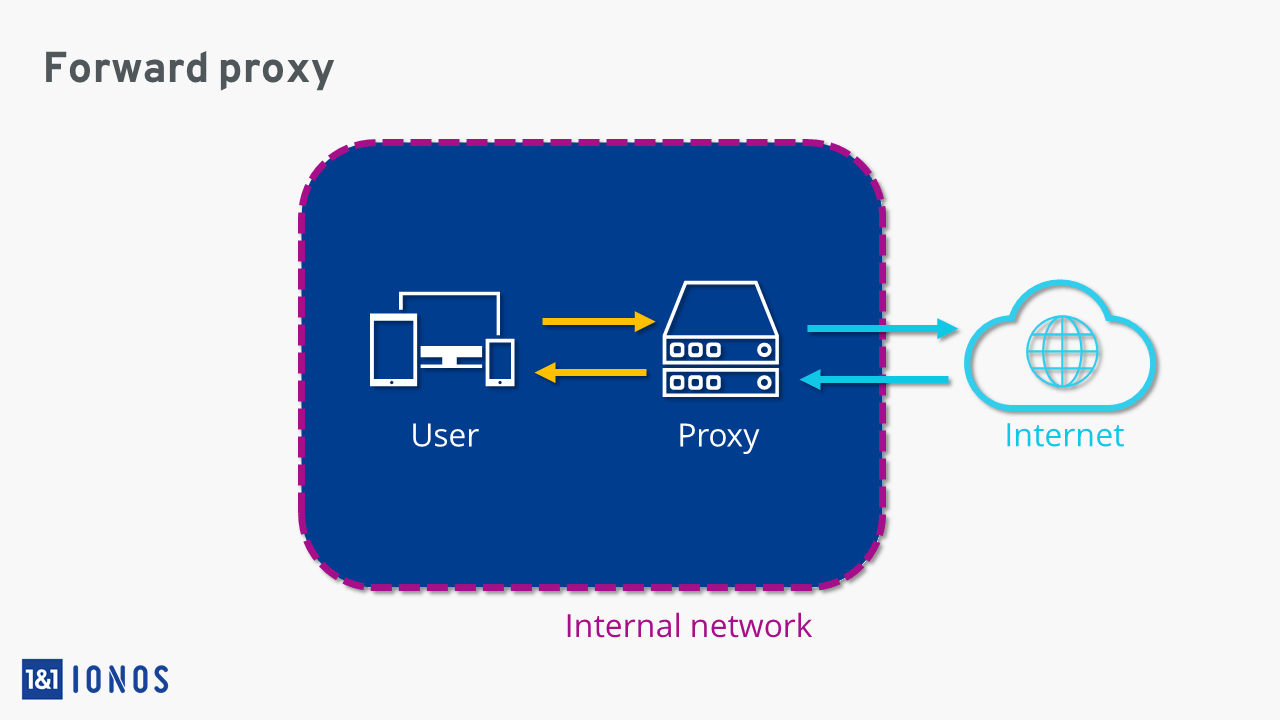
\includegraphics[width=0.49\textwidth]{imagenes/proxy}
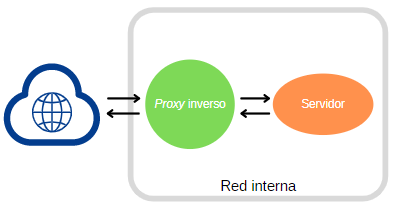
\includegraphics[width=0.49\textwidth]{imagenes/proxyInverso}
\caption{Esquema de un \emph{proxy} frente a un \emph{proxy} inverso.}
	\label{proxyContraProxyInverso}
\end{figure}

El uso de un \emph{proxy} inverso no queda restringido a ciertas arquitecturas, pudiéndose utilizar para ocultar el servicio o servicios que consume cualquier aplicación. Sin embargo, este componente adquiere una gran importancia en el enfoque de microservicios, pues es importante no exponer estos al exterior. Además, se suele utilizar también para realizar tareas de balanceo de carga entre diferentes instancias de un mismo microservicio. La figura \ref{proxyInversoContraNoProxyInverso} muestra la comparativa de una arquitectura de microservicios básica y otra que utiliza un \emph{proxy} inverso. En la segunda se observa que, con el uso de un componente de este tipo, los clientes no acceden directamente a los microservicios, ni siquiera los conocen.

\begin{figure}[ht]
\centering
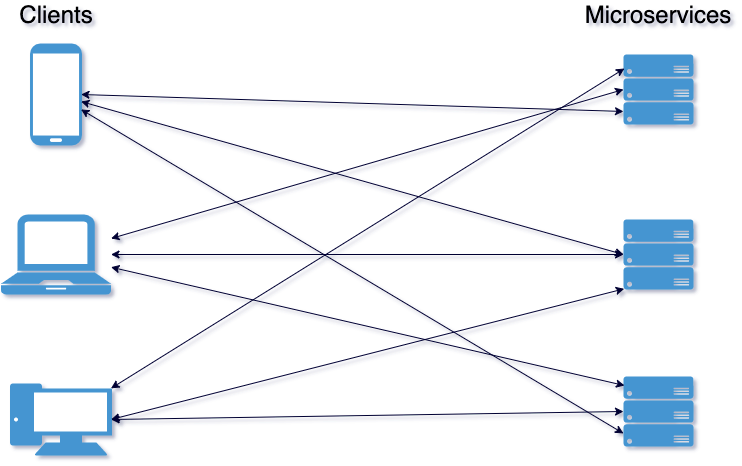
\includegraphics[width=0.49\textwidth]{imagenes/arquitecturaMicroserviciosBasica}
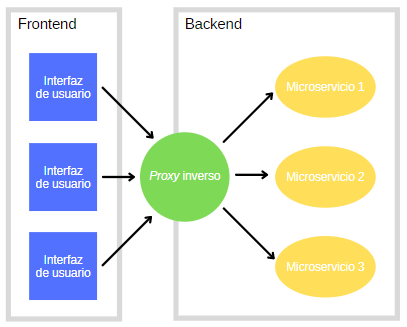
\includegraphics[width=0.49\textwidth]{imagenes/arquitecturaMicroserviciosConProxyInverso}
\caption{Arquitectura de microservicios básica frente a una con \emph{proxy} inverso.}
	\label{proxyInversoContraNoProxyInverso}
\end{figure}

Este proyecto surge en el contexto de una práctica en empresa. El autor ha tenido la oportunidad de formar parte del equipo de I+D+i de una empresa de desarrollo de software enfocada al sector sociosanitario, durante un periodo de tiempo de más de un año. Esta empresa comercializa un software de gestión de residencias y actualmente está desarrollando la nueva versión de su producto, utilizando enfoques y tecnologías de vanguardia. Entre ellos: arquitecturas de microservicios, desarrollo de software dirigido por modelos y generación automática de código.

La temática comentada fue elegida debido a la estrecha relación que guarda con el desempeño del autor en las prácticas mencionadas, esto es, contribuciones a un microservicio específico destinado a orquestar el despliegue de la aplicación de una forma automatizada. Por otro lado, el desarrollo a llevar a cabo le va a otorgar una visión más global de la aplicación sobre la que se trabaja, así como aumentar el nivel de conocimiento acerca de la misma, con la motivación de seguir contribuyendo al proyecto por mucho tiempo más. Por último, la tecnología a utilizar, .NET, es de su interés y aspira así a crecer como desarrollador de ese \emph{framework}.

	%%%%%%%%%%%%%%%%%%%%%%%%%%%%%% OBJETIVOS %%%%%%%%%%%%%%%%%%%%%%%%%%%%%%

	\section{Objetivos}

El objetivo principal de este trabajo es construir un \emph{proxy} inverso para una aplicación con arquitectura de microservicios. Su elaboración tiene las siguientes aspiraciones sobre el producto en desarrollo:

\begin{itemize}

	\item \textbf{Ocultar los microservicios} que forman el \emph{backend} de la aplicación para que la interfaz de usuario no acceda directamente a ellos por motivos de seguridad.

	\item Permitir la ejecución simultánea de \textbf{múltiples instancias} de los microservicios, que será fruto de:

	\begin{itemize}

		\item \textbf{Desacoplar los microservicios} entre ellos y evitar que cada uno tenga que conocer donde se encuentra el resto.

	\end{itemize}	

	y, a su vez, tiene por finalidad:

	\begin{itemize}

		\item Conseguir que la aplicación sea \textbf{tolerante a fallos}, gracias a la posibilidad de tener un mismo microservicio desplegado en máquinas diferentes.

		\item \textbf{Aumentar la eficiencia}, al poder crear o parar instancias dinámicamente según el tráfico que reciba la aplicación.

	\end{itemize}

\end{itemize}

	%%%%%%%%%%%%%%%%%%%%%%%%%%%%%% ESTRUCTURA DEL DOCUMENTO %%%%%%%%%%%%%%%%%%%%%%%%%%%%%%

	\section{Estructura del documento}

Este documento se divide en 5 grandes bloques o capítulos:

\begin{itemize}

	\item El primero de ellos es este y en él se introduce el trabajo realizado a través de la motivación del mismo, los objetivos a cumplir y esta presentación de la estructura de la memoria.

	\item En el capítulo 2 se expone un breve estado del arte para revisar las soluciones posibles al problema que implica a este trabajo, así como una comparativa de dichas propuestas.

	\item El capítulo número 3 comenta la tecnología que finalmente ha sido utilizada, justificando su elección y mostrando un ejemplo básico de su uso.

	\item El cuarto capítulo es el más extenso y comenta el proceso que se ha seguida para desarrollar el \emph{proxy} inverso. Incluye la especificación de requisitos, el diseño de la solución, la metodología seguida, las funcionalidades implementadas en un apartado dedicado a la programación y las pruebas realizadas.

	\item Por último, el capítulo 5 hace una reflexión sobre el trabajo realizado y concluye la misma valorando el grado de cumplimiento de los objetivos planteados. También presenta el trabajo futuro a realizar.

\end{itemize}

Como recurso adicional, se presenta un apéndice que explica el proceso de generación de código a partir de modelos que se ha utilizado para construir el \emph{proxy} inverso, en concreto, y los microservicios de la aplicación de la que forma parte, en general.

%%%%%%%%%%%%%%%%%%%%%%%%%%%%%% ESTADO DEL ARTE %%%%%%%%%%%%%%%%%%%%%%%%%%%%%%

\chapter{Estado del arte}

En la actualidad existen en el mercado muchas aplicaciones y servicios que se pueden utilizar como \emph{proxy} inverso. Algunas de estas soluciones son de pago, otras gratuitas e incluso algunas de código abierto. Se pueden dividir en dos tipos: productos \emph{software} ya construidos y librerías. Los primeros suelen ser fáciles de configurar y se pueden poner en marcha de una manera muy rápida. Las segundas requieren una parte de programación pero se adaptan mejor a las necesidades particulares, pues permiten tener más control al usuario. A continuación se van a comentar dos herramientas de cada tipo, una de las cuales será la escogida para desarrollar el \emph{proxy} inverso. Se hablará de la tecnología utilizada en general y de su elección en el siguiente capítulo (\ref{tecnologiaUtilizada}), donde también se mostrará un ejemplo básico de su uso.

Cabe destacar que no hay muchos productos que se dediquen exclusivamente a funcionar como \emph{proxy} inverso. Estos suelen ofrecer otros servicios como servidores web o balanceadores de carga. Por otro lado, lo habitual es hacer uso de un producto ya hecho, por lo que tampoco es fácil encontrar librerías que permitan personalizar un \emph{proxy} inverso, menos aún si hay que tener en cuenta la tecnología que se quiere utilizar. En relación con esto, las librerías elegidas son para ASP.NET Core \cite{DotNetCore}, tecnología empleada en el resto de la aplicación de la que forma parte el \emph{proxy} inverso.

	%%%%%%%%%%%%%%%%%%%%%%%%%%%%%% API GATEWAY %%%%%%%%%%%%%%%%%%%%%%%%%%%%%%

	\section{Patrón API \emph{Gateway}}

A modo de aparte, es interesante mencionar un patrón parecido al \emph{proxy} inverso y que también podría haber sido utilizado para resolver el problema que atañe a este trabajo: el API \emph{Gateway} \cite{ApiGateway}, o puerta de enlace de API. Ambos comparten algunos casos de uso, por lo que sus diferencias causan confusión y no suelen quedar claras.

Generalmente, se entiende que un API \emph{Gateway} es una especialización de un \emph{proxy} inverso, proporcionando así funcionalidades extra. Las más aceptadas e importantes son:

\begin{itemize}
	
	\item Suelen ofrecer agregaciones de peticiones, esto es, aunar dos o más llamadas al \emph{backend} y exponer esta composición a través de un único \emph{endpoint}.
	
	\item Realizan tareas transversales a todos los \emph{endpoints} como autenticación, autorización o monitorización.

	\item Interpretan los mensajes que reciben y pueden hacer transformaciones sobre ellos, mientras que los \emph{proxy} inversos solo los redirigen donde corresponda.

\end{itemize}

Este patrón fue descartado desde el primer momento porque no se quería tener la funcionalidad de ninguno de los tres puntos clave que caracterizan esta aproximación. Por este motivo, y por la búsqueda de sencillez, ha sido más apropiado decantarse por un \emph{proxy} inverso, de ahí que las tecnologías expuestas a continuación sean las que son.

	%%%%%%%%%%%%%%%%%%%%%%%%%%%%%% PRODUCTOS HECHOS %%%%%%%%%%%%%%%%%%%%%%%%%%%%%%

	\section{Productos}

		%%%%%%%%%%%%%%%%%%%%%%%%%%%%%% NGINX %%%%%%%%%%%%%%%%%%%%%%%%%%%%%%

		\subsection{NGINX}

Originariamente NGINX \footnote{Web oficial de NGINX: \url{https://www.nginx.com}.} fue construido para ser un servidor web pero más tarde ofreció la posibilidad de actuar como \emph{proxy} inverso, balanceador de carga o incluso \emph{proxy} para protocolos de correo electrónico, entre otros. De este modo, NGINX brinda muchos productos, con un conjunto de servicios cada uno. Se muestran los principales en la figura \ref{productosNGINX}. Los dos más utilizados son NGINX Open Source y NGINX Plus. El primero de ellos ofrece un servidor web \emph{open} source mientras que el segundo es de pago y permite utilizar un API \emph{Gateway} o un \emph{proxy} inverso.

\begin{figure}[ht]
\centering
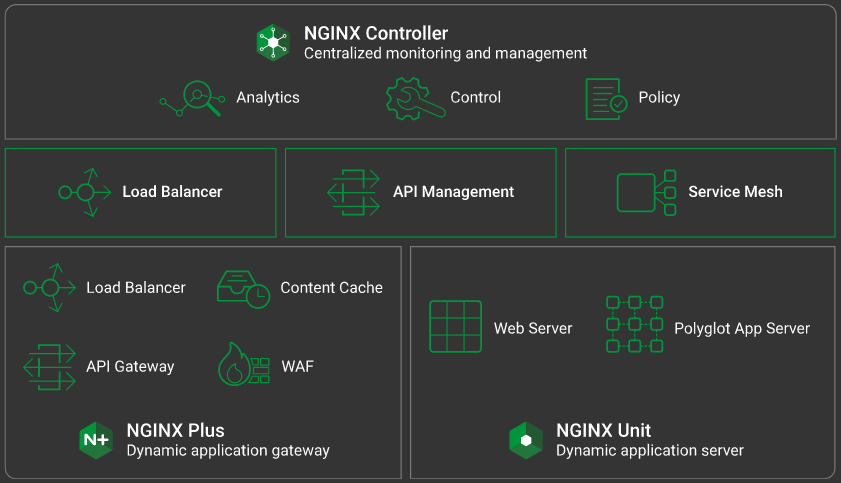
\includegraphics[width=0.9\textwidth]{imagenes/productosNGINX}
\caption[Productos NGINX.]{Productos NGINX \cite{NGINX}.}
	\label{productosNGINX}
\end{figure}

Desde la vertiente que interesa a este trabajo, se trata de un \emph{proxy} inverso ligero y de alto rendimiento. Sin embargo, no es uno de los servicios más utilizados de NGINX, por lo que no cuenta con muchas funcionalidades ni se puede personalizar en exceso. Las características más importantes que ofrece son transformaciones de \emph{headers}, configuración de \emph{buffers} a modo de memoria caché y creación de reglas de enrutamiento en base a las direcciones origen de las peticiones.

Se configura a través de un fichero el cual puede ser recargado durante su ejecución, es decir, se puede configurar dinámicamente. Un ejemplo de este lo muestra la figura \ref{configuracionNGINX}.

\begin{figure}[ht]
\centering
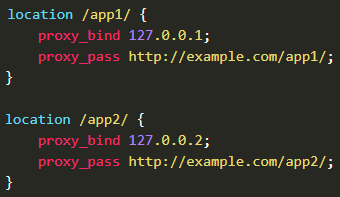
\includegraphics[width=0.5\textwidth]{imagenes/configuracionNGINX}
\caption[Ejemplo de configuración de NGINX.]{Ejemplo de configuración de NGINX \cite{NGINX_documentacion}.}
	\label{configuracionNGINX}
\end{figure}

Para finalizar, algunos de los productos y servicios de NGINX son ampliamente conocidos y utilizados por empresas de todo el mundo, entre ellas: Starbucks \footnote{Web oficial de Starbucks: \url{https://www.starbucks.es}.}, Bank of America \footnote{Web oficial de Bank of America: \url{https://www.bankofamerica.com}.} o Capital One \footnote{Web oficial de Capital One: \url{https://www.capitalone.com}.}. No obstante, su función de \emph{proxy} inverso no es una de ellas, como ya se ha comentado.

		%%%%%%%%%%%%%%%%%%%%%%%%%%%%%% KEMP %%%%%%%%%%%%%%%%%%%%%%%%%%%%%%

		\subsection{Kemp}

Kemp \footnote{Web oficial de Kemp: \url{https://kemptechnologies.com}.} es un balanceador de carga muy utilizado a nivel mundial. El término balanceador de carga se refiere a un \emph{proxy} inverso al que se le quiere dar énfasis a su capacidad de distribuir la carga entre varios nodos. Por esta característica es por la que se suele utilizar un producto de este tipo pero no hay que obviar que no deja de ser un \emph{proxy} inverso, con todo lo que conlleva.

En cuanto a sus características, ofrece ser un balanceador de nivel 4 pero también de nivel 7. Esto hace referencia a la capa del Modelo OSI (figura \ref{modeloOSI}) sobre la que actúa. Además, soporta HTTP/2, cuenta con un \emph{firewall} que se puede activar y tiene un mecanismo de \emph{health checks} para comprobar el estado de los \emph{endpoints} con los que trabaja.

Una de los aspectos más especiales de Kemp es el hecho de que brinda múltiples opciones de implementación, y muy flexibles. Destacan la \emph{hardware}, que facilita la instalación de máquinas con el \emph{software} de Kemp, y la \emph{cloud}, la cual pone a disposición los servicios de manera remota y sin necesidad tener servidores físicos. Cada una de ellas tiene diferentes tarifas en función del tráfico a recibir o de la cantidad de puertos disponibles, entre otros.

El precio por utilizar los servicios de Kemp varía en función de las características del proyecto en el que se quiere incluir. Hay que rellenar un pequeño cuestionario para recibir un presupuesto. En él, hay que indicar cosas como los productos que se quiere contratar y la cantidad de los mismos.

\begin{figure}[ht]
\centering
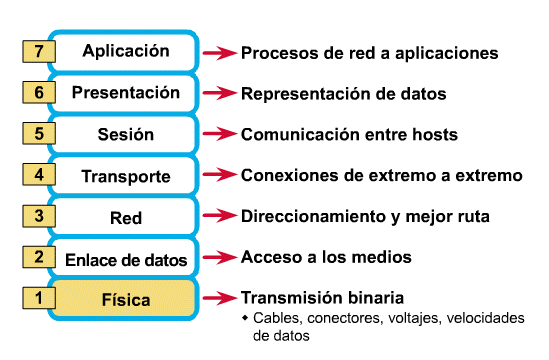
\includegraphics[width=0.8\textwidth]{imagenes/modeloOSI}
\caption[Modelo OSI.]{Modelo OSI \cite{OSI}.}
	\label{modeloOSI}
\end{figure}

Ejemplos de empresas que utilizan Kemp en sus infraestructuras son Audi \footnote{Web oficial de Audi: \url{https://www.audi.es}.}, Nestle \footnote{Web oficial de Nestle: \url{https://www.nestle.com}.} o Galp \footnote{Web oficial de Galp: \url{https://www.galpenergia.com/}.}.

	%%%%%%%%%%%%%%%%%%%%%%%%%%%%%% LIBRERÍAS %%%%%%%%%%%%%%%%%%%%%%%%%%%%%%

	\section{Librerías}

		%%%%%%%%%%%%%%%%%%%%%%%%%%%%%% YARP %%%%%%%%%%%%%%%%%%%%%%%%%%%%%%

		\subsection{YARP}

YARP \footnote{Web oficial de YARP: \url{https://microsoft.github.io/reverse-proxy}.} es una librería para ASP.NET Core hecha por el propio Microsoft \footnote{Web oficial de Microsoft: \url{https://www.microsoft.com}.} y su objetivo es facilitar la creación de \emph{proxy} inversos. Surgió dentro de la propia infraestructura de la empresa, en la que diferentes equipos preguntaban si existía algún producto de este tipo disponible para utilizar en sus respectivos proyectos. La respuesta de la compañía fue crear un equipo especializado para construir esta librería y estandarizar así su uso. Además, se decidió hacer pública tanto su existencia como su código, siendo así una opción \emph{open source} a tener en cuenta.

Se encuentra todavía en desarrollo, habiendo sido lanzada su primera \emph{release} el 25 de Junio de 2020, y, a fecha de este trabajo, todavía solo se puede utilizar una \emph{preview}. Se prevé que vayan saliendo a la luz más versiones con más funcionalidades basadas en la experiencia de la propia empresa pero también en las opiniones de los usuarios externos. YARP es compatible con .NET Core 3.1 y .NET 5 pero algunas funcionalidades solo están disponibles para el segundo \emph{framework}, ya que se trata de la generación inmediatamente más moderna.

A raíz de la heterogeneidad de casos de uso que debe cubrir para satisfacer las necesidades de los diferentes equipos de Microsoft, está diseñada para ser muy personalizable y flexible. Otro aspecto importante es que permite cambiar la configuración del \emph{proxy} inverso de forma dinámica, lo que no obliga a tener que volver a lanzarlo a ejecución cuando se añada una nueva ruta, por ejemplo.

Permite construir \emph{proxy} inversos de nivel 7, la capa de aplicación en este caso. Gracias a esto, es posible modificar una petición HTTP antes de redirigirla, como por ejemplo sus \emph{headers} o ruta de destino. Sin embargo, no se puede hacer lo mismo con su contenido, ni siquiera es interpretado para tardar el menor tiempo posible en redirigir las peticiones. Además, no es un componente aparte sino que se integra con la \emph{pipeline} de \emph{middlewares} de ASP.NET \cite{MiddlewaresPipeline}, haciendo que su eficiencia sea muy alta.

Por último, la documentación propia no es escueta pero tampoco excesiva. Asimismo, su corta edad hace que no se encuentren referencias o ejemplos de código de la comunidad fácilmente. Tampoco problemas planteados con sus posibles soluciones en portales como Stack Overflow \footnote{Web oficial de Stack Overflow: \url{https://es.stackoverflow.com}.}.

		%%%%%%%%%%%%%%%%%%%%%%%%%%%%%% OCELOT %%%%%%%%%%%%%%%%%%%%%%%%%%%%%%

		\subsection{Ocelot}

Ocelot \footnote{Web oficial de Ocelot: \url{https://threemammals.com/ocelot}.} es una librería para ASP.NET Core que permite a una aplicación de ese \emph{framework} actuar como API \emph{Gateway}. Como su propia web dice, está pensada para arquitecturas orientadas a servicios o a microservicios que necesitan un punto único de entrada.

Se trata de un proyecto que ya tiene cierto tiempo, pues se inició en 2016. No obstante, su última \emph{release} salió a la luz el 11 de Diciembre de 2020 y es compatible con la última versión de .NET, .NET 5. También lo es con todas las anteriores de .NET Core.

En lo que se refiere a las características propias de API \emph{Gateway}, Ocelot ofrece agregación de peticiones y tareas comunes a todos los \emph{enpoints} como autenticación o trazas distribuidas. También puede hacer transformaciones de \emph{headers} o cambiar el método HTTP utilizado antes de redirigir una petición.

Otra de sus características destacables son el hecho de ser \emph{open source}, su rapidez y su escalabilidad. También es conveniente comentar que puede proporcionar autenticación, descubrimiento de servicios, equilibrio de carga, cacheado y limitación de carga. En sus inicios, uno de sus peores puntos negativos era que no permitía cambiar su configuración de manera dinámica, sin embargo, esta característica fue añadida más tarde y ahora ya está disponible.

Al igual que YARP, Ocelot también está formado por una serie de \emph{middlewares} que se integran en la pipeline de ASP.NET para llevar a cabo sus tareas de API \emph{Gateway}. Su configuración es muy básica, teniendo que especificarla en un fichero Json. La figura \ref{configuracionBasicaOcelot} muestra un ejemplo muy básico de este fichero y la figura \ref{configuracionAgregacionOcelot} uno con una agregación de peticiones. De estos ejemplos es interesante comentar la nomenclatura que utiliza esta librería para diferenciar el flujo de entrada de peticiones (\emph{upstream}) del de salida (\emph{downstream}). Por último, en el segundo ejemplo se observa lo sencillo que es configurar agregaciones de peticiones, indicando un identificador, la ruta base de peticiones a capturar y los identificadores de las rutas que agregar.

\begin{figure}[ht]
\centering
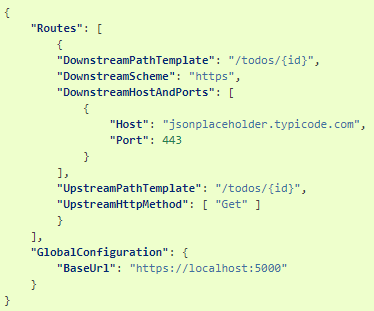
\includegraphics[width=0.7\textwidth]{imagenes/configuracionBasicaOcelot}
\caption[Ejemplo básico de configuración de Ocelot.]{Ejemplo básico de configuración de Ocelot \cite{Ocelot_documentacion}.}
	\label{configuracionBasicaOcelot}
\end{figure}

\begin{figure}[ht]
\centering
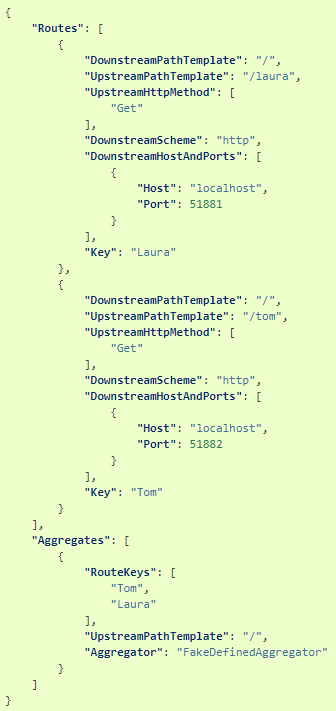
\includegraphics[width=0.6\textwidth]{imagenes/configuracionAgregacionOcelot}
\caption[Ejemplo de configuración de Ocelot con una agregación de peticiones.]{Ejemplo de configuración de Ocelot con una agregación de peticiones \cite{Ocelot_documentacion}.}
	\label{configuracionAgregacionOcelot}
\end{figure}

	%%%%%%%%%%%%%%%%%%%%%%%%%%%%%% COMPARATIVA %%%%%%%%%%%%%%%%%%%%%%%%%%%%%%

	\section{Comparativa}

Precio, API Gateway, Reverse proxy, documentación, comunidad, previa configuración, cantidad de posible configuración, extensibilidad, recarga de configuración dinámica, capa modelo OSI.

	%%%%%%%%%%%%%%%%%%%%%%%%%%%%%% CONCLUSIONES %%%%%%%%%%%%%%%%%%%%%%%%%%%%%%

	\section{Conclusiones}

Conveniencia de la realización de este trabajo.

%%%%%%%%%%%%%%%%%%%%%%%%%%%%%% TECNOLOGÍA UTILIZADA %%%%%%%%%%%%%%%%%%%%%%%%%%%%%%

\chapter{Tecnología utilizada} \label{tecnologiaUtilizada}

La tecnología utilizada es .NET \cite{DotNet}, más concreto, ASP.NET Core \cite{DotNetCore}, con el lenguaje de programación C\# \cite{Csharp} y el entorno de desarrollo habitual para él, Visual Studio \footnote{Web oficial de Visual Studio: \url{https://visualstudio.microsoft.com/es/vs}.}, en la versión del 2019. Como se comenta en la introducción del capítulo anterior, la aplicación en la cual se incluye el \emph{proxy} inverso está construida con ese \emph{framework}, por lo que se quiso mantener ese aspecto también en el nuevo componente. Esto corresponde al requisito no funcional RNF03, que se verá en el apartado \ref{requisitosNoFuncionales}.

Por otro lado, se ha decidido utilizar YARP para construir el \emph{proxy} inverso. La aplicación sobre la que se trabaja posee un mecanismo de despliegue automático muy 
particular, por lo que la flexibilidad y capacidad de adaptación que ofrece esta librería son muy adecuadas para integrar el \emph{proxy} inverso con dicho proceso. Si se hubiera utilizado un producto ya hecho, no se hubiera podido conseguir un nivel alto de cohesión y se hubieran tenido que abordar problemas de integración. Por otro lado, su sencillez y altas prestaciones hacen que destaque frente a Ocelot, la que, como ya se ha comentado, permite crear API \emph{Gateways}.

Por último, se ha utilizado Postman \footnote{Web oficial de Postman: \url{https://www.postman.com}.} para realizar consultas de prueba al \emph{proxy} inverso y comprobar su funcionamiento. Postman es una herramienta gratuita que permite hacer justo lo que se ha descrito. Se trata de un cliente para peticiones HTTP REST que se utiliza para probar de manera sencilla servicios web y así agilizar su desarrollo.

	%%%%%%%%%%%%%%%%%%%%%%%%%%%%%% EJEMPLO DE USO BÁSICO DE YARP %%%%%%%%%%%%%%%%%%%%%%%%%%%%%%

	\section{Ejemplo de uso básico de YARP} \label{ejemploUsoYARP}

Una vez comentada la elección que finalmente se hizo y el porqué, se va a introducir un ejemplo de uso básico de YARP para dar una visión general de lo que es capaz de hacer esta librería. De este modo, también será más fácil comprender el funcionamiento del \emph{proxy} inverso desarrollado.

En lineas generales, empezar a utilizar YARP no es nada difícil, en un par de horas se puede llegar a tener un \emph{proxy} inverso básico funcionando. Si bien, es más complejo utilizar características avanzadas o personalizarlo en función de las necesidades particulares.

La demostración que se va a realizar consiste en crear un \emph{proxy} inverso que redirija peticiones hacía dos servicios web de prueba, creados anteriormente para el ejemplo. Estos simulan ser un servicio de localización y devuelven siempre ''\emph{Valencia, Spain}''. También muestran este mismo mensaje por consola cuando son consultados para poder visualizar a través de ella la cantidad de peticiones que responden.

Para empezar con el ejemplo, se crea un proyecto web vacío de .NET, en concreto, de ASP.NET Core. Una vez el proyecto se ha creado, hay que añadir la referencia a la librería de YARP. En .NET las librerías se añaden como paquete NuGet \cite{NuGet} y para buscar qué paquetes hay disponibles e instalarlos se puede utilizar un asistente gráfico, figura \ref{ejemploYARP_instalacionNuGet}.

\begin{figure}[ht]
\centering
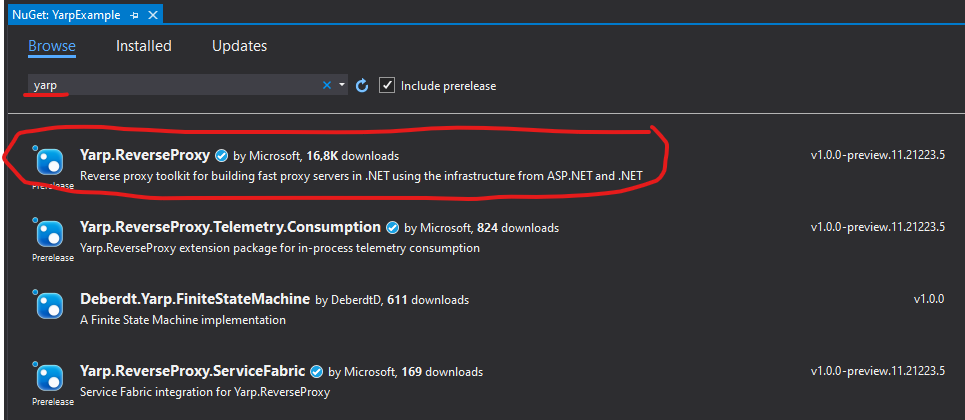
\includegraphics[width=1\textwidth]{imagenes/ejemploYARP/instalacionNuGet}
\caption{Instalación del NuGet de YARP.}
	\label{ejemploYARP_instalacionNuGet}
\end{figure}

Acto seguido, es necesario añadir un poco de código para poner en marcha un \emph{proxy} inverso sencillo. En la clase \emph{Startup} hay que modificar los métodos por defecto \emph{ConfigureServices} y \emph{Configure}. En el primero de ellos es necesario registrar el código del \emph{proxy} inverso, haciendo \emph{services.AddReverseProxy()}, y cargar la configuración de las rutas, \emph{proxyBuilder.LoadFromConfig()}. En el segundo basta con asegurarse de que se haga la llamada \emph{app.UseRouting()} y añadir  \emph{MapReverseProxy()} dentro del \emph{UseEndpoint}. Para visualizar mejor estos cambios, figura \ref{ejemploYARP_startup}.

\begin{figure}[ht]
\centering
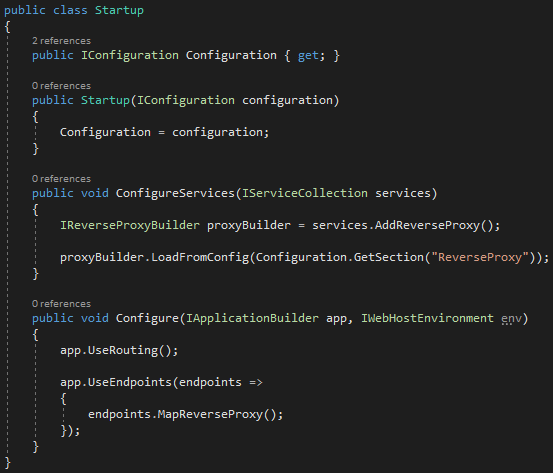
\includegraphics[width=0.8\textwidth]{imagenes/ejemploYARP/startup}
\caption{Clase \emph{Startup} después de añadir el código del \emph{proxy} inverso.}
	\label{ejemploYARP_startup}
\end{figure}

Por otro lado, hay que configurar las rutas que va a tener el \emph{proxy} inverso, es decir, los enrutamientos que debe hacer en tiempo de ejecución. Para ello se necesita especificar dichas rutas en el archivo \emph{appsettings.json}. Este archivo se utiliza para especificar cualquier tipo de configuración y se podría haber utilizado otro diferente. También se puede configurar a través de código pero requiere algo más de trabajo. Por este motivo, en esta demostración se va a utilizar el primer método, ya que se pretende mostrar un ejemplo lo más simple posible.

La figura \ref{ejemploYARP_appsettings} muestra las rutas creadas para esta prueba. Se ha creado un par ruta-\emph{cluster} con dos destinaciones. Para no entrar en mucho detalle, lo que es importante es que la ruta tiene un patrón \emph{\{**catch-all\}} dentro de la cláusula \emph{Match:Path}, para capturar todas las peticiones, y el \emph{cluster} contiene dos destinaciones, una por cada servicio de localización, comentados al principio de este apartado. Lo que se pretende conseguir con esta configuración es que el \emph{proxy} inverso capture todas las peticiones y las envíe de manera aleatoria a cualquiera de los dos servicios.

\begin{figure}[ht]
\centering
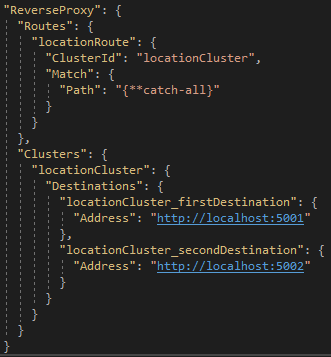
\includegraphics[width=0.5\textwidth]{imagenes/ejemploYARP/appsettings}
\caption{Fichero \emph{appsettings.json} con la configuración de las rutas para el \emph{proxy} inverso.}
	\label{ejemploYARP_appsettings}
\end{figure}

Lo siguiente es preparar los servicios para una prueba rápida. En la figura \ref{ejemploYARP_servicios_preparacion} se observa el escenario inicial. En la parte superior se encuentra el \emph{proxy} inverso creado y, en la inferior, los dos servicios de localización . Importante destacar que los puertos de estos últimos coinciden con los que se han indicado en el \emph{appsettings.json}.

\begin{figure}[ht]
\centering
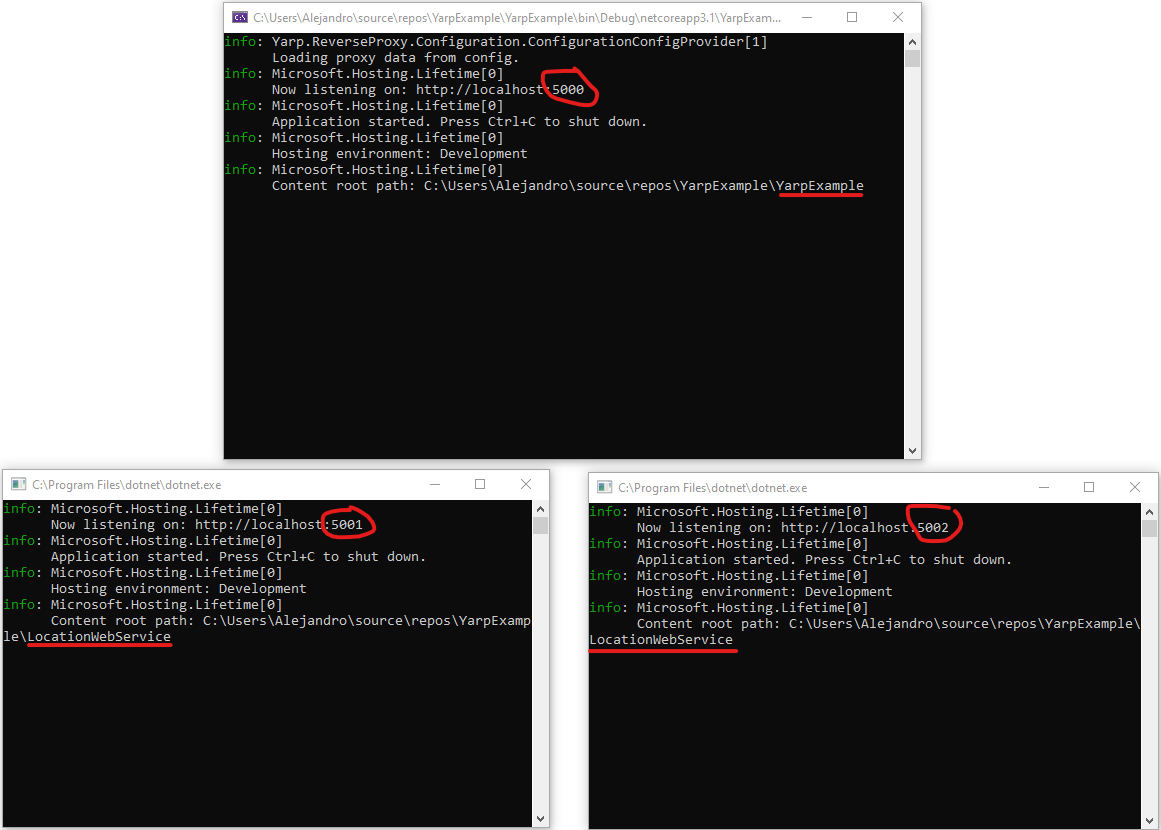
\includegraphics[width=1\textwidth]{imagenes/ejemploYARP/servicios_preparacion}
\caption{Escenario inicial de prueba de YARP con los servicios preparados.}
	\label{ejemploYARP_servicios_preparacion}
\end{figure}

Para simular una petición de un cliente se va a realizar una consulta con Postman. Esta estará dirigida al \emph{proxy} inverso y deberá ser redirigida a alguno de los dos servicios de localización, como se ha configurado en el \emph{appsettings.json}. En la figura \ref{ejemploYARP_servicios_funcionando}, se muestra el escenario anterior tras ejecutar la petición Postman repetidas veces. Se observa que el \emph{proxy} inverso la ha redirigido de manera aleatoria entre los dos otros servicios. En la consola del \emph{proxy} inverso es interesante ver el mensaje por defecto que muestra YARP indicando hacia qué dirección redirige cada petición.

\begin{figure}[ht]
\centering
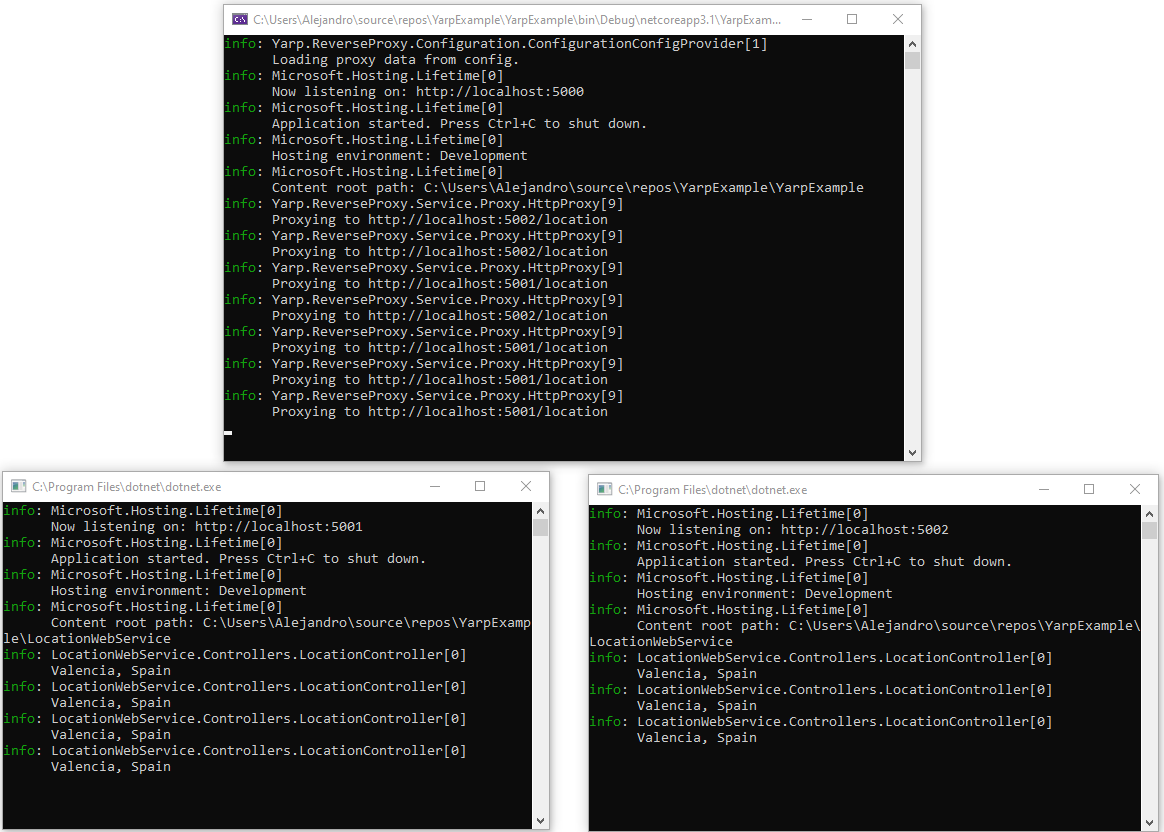
\includegraphics[width=1\textwidth]{imagenes/ejemploYARP/servicios_funcionando}
\caption{Escenario de prueba de YARP con los servicios después de realizar algunas consultas.}
	\label{ejemploYARP_servicios_funcionando}
\end{figure}

%%%%%%%%%%%%%%%%%%%%%%%%%%%%%% DESARROLLO DE LA SOLUCIÓN %%%%%%%%%%%%%%%%%%%%%%%%%%%%%%

\chapter{Desarrollo de la solución}

Este capítulo va a explicar el proceso que se ha seguido para construir el \emph{proxy} inverso. Primero se detallará la funcionalidad que este debe tener mediante la especificación de requisitos previa al desarrollo. En segundo lugar, se verá una sección de diseño para ver cómo se organiza el código de la solución implementada. A continuación, se explicará la metodología \emph{software} seguida. Después, la sección más amplia, correspondiente a la programación del \emph{proxy} inverso, la cual se comentará divida en fases con las funcionalidades implementadas en cada una de ellas y los problemas encontrados. Por último, se expondrán las pruebas realizadas para verificar el correcto funcionamiento del producto elaborado.

	%%%%%%%%%%%%%%%%%%%%%%%%%%%%%% ESPECIFICACIÓN DE REQUISITOS %%%%%%%%%%%%%%%%%%%%%%%%%%%%%%

	\section{Especificación de requisitos} \label{especificacionRequisitos}

La especificación de requisitos del \emph{proxy} inverso se ha llevado a cabo elaborando los casos de uso que debe cubrir. Adicionalmente a estos, también se expondrán otros requisitos funcionales y no funcionales que el producto debe satisfacer.

		%%%%%%%%%%%%%%%%%%%%%%%%%%%%%% CASOS DE USO %%%%%%%%%%%%%%%%%%%%%%%%%%%%%%

		\subsection{Casos de uso} \label{casosDeUso}

Los casos de uso van a ser expuestos a continuación con un diagrama de casos de uso, figura \ref{diagramaCasosDeUso}, y en formato de tabla, indicando para cada uno de ellos un identificador, un nombre, el actor que lo lleva a cabo y una breve descripción:

\begin{figure}[ht]
\centering
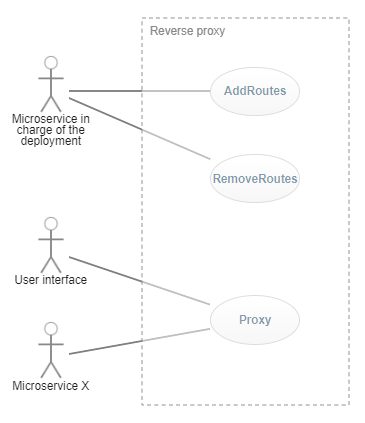
\includegraphics[width=0.52\textwidth]{imagenes/diagramaCasosDeUso}
\caption{Diagrama de casos de uso del \emph{proxy} inverso.}
	\label{diagramaCasosDeUso}
\end{figure}

\begin{center} \begin{tabular}{| l | p{11.3cm} |}
\hline
\textbf{Identificador} & CU01
\\ \hline
\textbf{Nombre} & Añadir rutas
\\ \hline
\textbf{Actor} & Microservicio encargado de orquestar el despliegue
\\ \hline
\textbf{Descripción} & El microservicio que organiza los despliegues de la aplicación le indica al \emph{proxy} inverso unas rutas para que las tenga en cuenta a la hora de redirigir peticiones, CU03. Las rutas son descritas mediante la ruta base de las peticiones que tiene que capturar y la dirección a la que redirigirlas.
\\ \hline \end{tabular} \end{center}

\begin{center} \begin{tabular}{| l | p{11.3cm} |}
\hline
\textbf{Identificador} & CU02
\\ \hline
\textbf{Nombre} & Eliminar rutas
\\ \hline
\textbf{Actor} & Microservicio encargado de orquestar el despliegue
\\ \hline
\textbf{Descripción} & El microservicio que organiza los despliegues de la aplicación le indica al \emph{proxy} inverso unas rutas para que las deje de tener en cuenta a la hora de redirigir peticiones, CU03. Las rutas son descritas mediante la ruta base de las peticiones que tiene que dejar de capturar y la dirección a la que no redirigir más peticiones.
\\ \hline \end{tabular} \end{center}

\begin{center} \begin{tabular}{| l | p{11.3cm} |}
\hline
\textbf{Identificador} & CU03
\\ \hline
\textbf{Nombre} & Enrutamiento
\\ \hline
\textbf{Actor} & Interfaz de usuario / Microservicio X
\\ \hline
\textbf{Descripción} & La interfaz de usuario o cualquier microservicio de la aplicación envía una petición a la dirección en la que escucha el \emph{proxy} inverso y esta es capturada y redirigida hacia un \emph{endpoint} especificado por una determinada ruta. Las rutas determinan qué peticiones tienen que ser encaminadas a qué direcciones. Es necesario cargar previamente la ruta correspondiente mediante el caso de uso CU01.
\\ \hline \end{tabular} \end{center}

		%%%%%%%%%%%%%%%%%%%%%%%%%%%%%% REQUISITOS FUNCIONALES %%%%%%%%%%%%%%%%%%%%%%%%%%%%%%

		\subsection{Otros requisitos funcionales} \label{requisitosFuncionales}

Aparte de los casos de uso comentados en el apartado anterior, el \emph{proxy} inverso ha de cumplir otros requisitos funcionales, o características concretas, que no son propiamente casos de uso pero que se considera de interés mencionarlos, pues son relevantes para su funcionamiento. Los requisitos funcionales a mostrar se centran en lo que debe hacer el sistema y dejan de lado la interacción con el usuario. Complementan así los casos de uso y ayudan también a comprender qué debe hacer exactamente el producto. Cabe destacar que estos aspectos se podrían haber presentado de forma conjunta a los casos de uso, ya que ambos se pueden considerar requisitos funcionales. No obstante, se cree que de esta manera quedan más claras, por un lado, las tres funcionalidades básicas y, por otro lado, algunos detalles más concretos.

Estos requisitos van a ser representados mediante un identificador, un nombre, el caso de uso con el que guardan relación, y una breve descripción:

\begin{center} \begin{tabular}{| l | p{9.5cm} |}
\hline
\textbf{Identificador} & RF01
\\ \hline
\textbf{Nombre} & Carga de rutas dinámica
\\ \hline
\textbf{Caso de uso relacionado} & CU01
\\ \hline
\textbf{Descripción} & La acción de añadir rutas a las que redirigir peticiones se debe poder hacer de manera dinámica, es decir, durante la propia ejecución. Esto permite no tener que parar y volver a lanzar el \emph{proxy} inverso cada vez que se añaden o eliminan rutas. Esta es una característica bastante importante ya que el tiempo en el que se reinicia no estaría atendiendo peticiones y estas fallarían, quedando el sistema inaccesible durante ese tiempo.
\\ \hline \end{tabular} \end{center}

\begin{center} \begin{tabular}{| l | p{9.5cm} |}
\hline
\textbf{Identificador} & RF02
\\ \hline
\textbf{Nombre} & Doble comunicación
\\ \hline
\textbf{Caso de uso relacionado} & CU03
\\ \hline
\textbf{Descripción} & El \emph{proxy} inverso tiene que estar preparado para servir de puerta de entrada al \emph{backend} desde la interfaz de usuario pero también debe interconectar los microservicios que forman dicho \emph{backend}. De esta forma, todas las peticiones que se lleven a cabo desde fuera o dentro del propio sistema deben pasar por él.
\\ \hline \end{tabular} \end{center}

\begin{center} \begin{tabular}{| l | p{9.5cm} |}
\hline
\textbf{Identificador} & RF03
\\ \hline
\textbf{Nombre} & Multiinstancia de microservicios
\\ \hline
\textbf{Caso de uso relacionado} & CU01, CU02 y CU03
\\ \hline
\textbf{Descripción} & Se debe soportar la ejecución simultánea de más de una instancia de un mismo microservicio, es decir, el \emph{proxy} inverso debe ser capaz de permitir la existencia de más de una dirección que atienda un mismo grupo de peticiones.
\\ \hline \end{tabular} \end{center}

\begin{center} \begin{tabular}{| l | p{9.5cm} |}
\hline
\textbf{Identificador} & RF04
\\ \hline
\textbf{Nombre} & Balanceo de carga
\\ \hline
\textbf{Caso de uso relacionado} & CU03
\\ \hline
\textbf{Descripción} & En relación con el RF03, las peticiones deben ser redirigidas de manera inteligente hacía las distintas direcciones posibles, si las hay, para una determinada ruta. En concreto, se busca no inundar de peticiones unas y dejar en el olvido otras.
\\ \hline \end{tabular} \end{center}

\begin{center} \begin{tabular}{| l | p{9.5cm} |}
\hline
\textbf{Identificador} & RF05
\\ \hline
\textbf{Nombre} & Versionado de microservicios
\\ \hline
\textbf{Caso de uso relacionado} & CU01, CU02 y CU03
\\ \hline
\textbf{Descripción} & Relacionado con el RF03, las diferentes instancias de un mismo microservicio pueden corresponder a versiones diferentes del mismo. De esta forma, las peticiones deberán ser redirigidas a una dirección u otra en función de la versión del microservicio que se quiera utilizar.
\\ \hline \end{tabular} \end{center}

\begin{center} \begin{tabular}{| l | p{9.5cm} |}
\hline
\textbf{Identificador} & RF06
\\ \hline
\textbf{Nombre} & Multiinstancia de \emph{proxy} inversos
\\ \hline
\textbf{Caso de uso relacionado} & CU03
\\ \hline
\textbf{Descripción} & Se debe poder trabajar con más de un \emph{proxy} inverso a la vez, de manera que uno enrute una petición hacía otro \emph{proxy} inverso y este segundo la enrute hacía el microservicio final. Este paso por más de un enrutador debe ser transparente para ellos, siendo su única función la de redirigir las peticiones.
\\ \hline \end{tabular} \end{center}

\begin{center} \begin{tabular}{| l | p{9.5cm} |}
\hline
\textbf{Identificador} & RF07
\\ \hline
\textbf{Nombre} & Instancias exclusivas
\\ \hline
\textbf{Caso de uso relacionado} & CU03
\\ \hline
\textbf{Descripción} & Derivado del RF06, debe ser posible desplegar un \emph{proxy} inverso que solo se encargue de las peticiones que vienen de la interfaz de usuario y otro para las que van de un microservicio a otro, pudiéndose aumentar el número de estos.
\\ \hline \end{tabular} \end{center}

		%%%%%%%%%%%%%%%%%%%%%%%%%%%%%% REQUISITOS NO FUNCIONALES %%%%%%%%%%%%%%%%%%%%%%%%%%%%%%

		\subsection{Requisitos no funcionales} \label{requisitosNoFuncionales}
		
Un requisito no funcional se entiende como una restricción impuesta sobre un producto \emph{software} que no corresponde a una funcionalidad del mismo. Están directamente relacionados con la calidad que tendrá el producto en cuestión y pueden referirse a características de diferentes tipos tales como fiabilidad o usabilidad. En concreto, la ISO/IEC 25010 \cite{ISO25010}, comúnmente llamada SQuaRE (\emph{System and software Quality Requirements and Evaluation}), define ocho características principales y algunas subcaracterísticas específicas para cada una. La figura \ref{iso25010} las muestra todas.

\begin{figure}[ht]
\centering
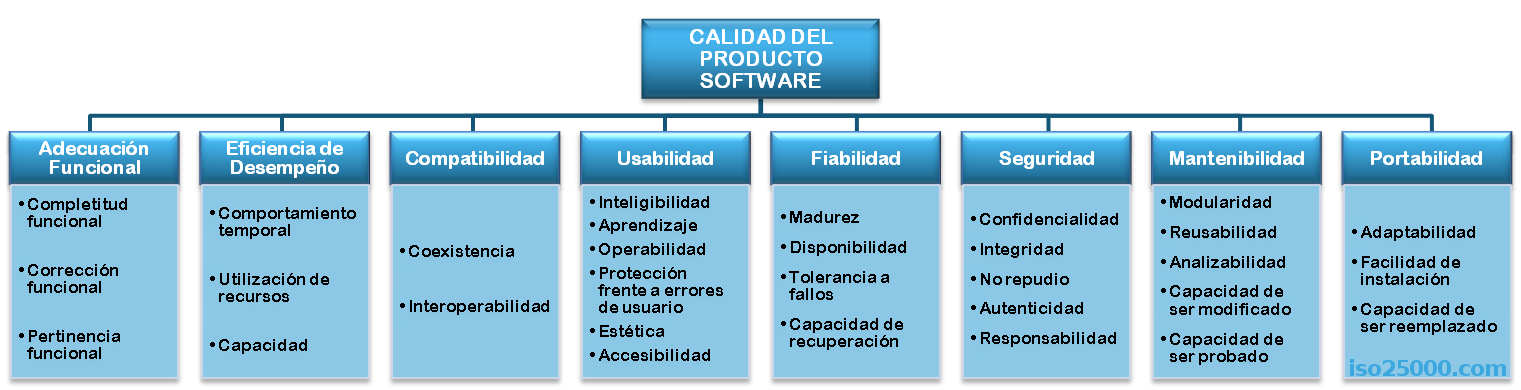
\includegraphics[width=1\textwidth]{imagenes/iso25010}
\caption[Características y subcaracterísticas de calidad de un producto \emph{software} definidas en la ISO/IEC 25010.]{Características y subcaracterísticas de calidad de un producto \emph{software} definidas en la ISO/IEC 25010 \cite{ISO25010}.}
	\label{iso25010}
\end{figure}

Sobre el \emph{proxy} inverso que atañe a este trabajo se imponen los siguientes requisitos no funcionales. Se detallan mediante un identificador, un nombre, la característica de la ISO a la que hacen referencia, una breve descripción y el motivo por el cual se considera necesario satisfacerlos:

\begin{center} \begin{tabular}{| l | p{11.3cm} |}
\hline
\textbf{Identificador} & RNF01
\\ \hline
\textbf{Nombre} & Autenticación de peticiones
\\ \hline
\textbf{Característica} & Seguridad
\\ \hline
\textbf{Descripción} & Se debe tener un sistema de autenticación que no permita escuchar ni redirigir peticiones sin autenticar. No se puede llevar a cabo ninguno de los tres casos de uso (CU01, CU02 y CU03) sin una previa autenticación.
\\ \hline
\textbf{Motivación} & Impedir que peticiones ajenas puedan ser atendidas y/o redirigidas para evitar posibles ataques.
\\ \hline \end{tabular} \end{center}

\begin{center} \begin{tabular}{| l | p{11.3cm} |}
\hline
\textbf{Identificador} & RNF02
\\ \hline
\textbf{Nombre} & Enrutamiento eficaz
\\ \hline
\textbf{Característica} & Eficiencia de desempeño
\\ \hline
\textbf{Descripción} & El enrutamiento, CU03, no debe ralentizar las peticiones en exceso de forma que las peticiones enrutadas no tomen un tiempo superior al 115\% del tiempo que tardaría la petición si no pasara por el \emph{proxy} inverso.
\\ \hline
\textbf{Motivación} & Evitar que el \emph{proxy} inverso suponga un retardo elevado en el tiempo de respuesta de las peticiones.
\\ \hline \end{tabular} \end{center}

\begin{center} \begin{tabular}{| l | p{11.3cm} |}
\hline
\textbf{Identificador} & RNF03
\\ \hline
\textbf{Nombre} & Tecnología impuesta
\\ \hline
\textbf{Característica} & Mantenibilidad
\\ \hline
\textbf{Descripción} & La tecnología a utilizar para llevar a cabo el proyecto tiene que ser .NET, con C\# como lenguaje de programación.
\\ \hline
\textbf{Motivación} & Guardar coherencia con el resto de los microservicios para poder ser mantenido por personas que hayan trabajado con otros de ellos anteriormente.
\\ \hline \end{tabular} \end{center}

\begin{center} \begin{tabular}{| l | p{11.3cm} |}
\hline
\textbf{Identificador} & RNF04
\\ \hline
\textbf{Nombre} & Estructura del proyecto
\\ \hline
\textbf{Característica} & Mantenibilidad
\\ \hline
\textbf{Descripción} & La estructura de carpetas y clases del proyecto debe ser similar a la de los demás microservicios, entendiéndose similar como aquella que pueda ser comprendida por una persona familiarizada con la estructura de referencia en un periodo de tiempo de 10 minutos como máximo.
\\ \hline
\textbf{Motivación} & Ídem RNF03: guardar coherencia con el resto de los microservicios para poder ser mantenido por personas que hayan trabajado con otros de ellos anteriormente.
\\ \hline \end{tabular} \end{center}

	%%%%%%%%%%%%%%%%%%%%%%%%%%%%%% DISEÑO %%%%%%%%%%%%%%%%%%%%%%%%%%%%%%

	\section{Diseño}

En lo que se refiere al diseño de la solución, se va presentar su estructura final. Por otro lado, también se cree conveniente comentar los \emph{middlewares} que forman la \emph{pipeline} de YARP para ver qué componentes personalizados han sido desarrollados y añadidos.

		%%%%%%%%%%%%%%%%%%%%%%%%%%%%%% ESTRUCTURA DE LA SOLUCIÓN %%%%%%%%%%%%%%%%%%%%%%%%%%%%%%

		\subsection{Estructura de la solución}

En el apartado \ref{requisitosNoFuncionales}, el requisito no funcional RNF04 impone que la estructura del \emph{proxy} inverso debe ser similar a la del resto de microservicios. Por este motivo, la estructura del producto final sigue esa referencia, que pasa a detallarse a continuación.

Un microservicio cualquiera de esta aplicación, y el \emph{proxy} inverso en particular, tiene una arquitectura autogenerada de 8 capas:

\begin{itemize}

	\item \textbf{Dominio}. En ella se encuentran las entidades que representan el dominio de la aplicación. Estas son creadas en base a su previo modelado.

	\item \textbf{Contratos}. Principalmente contiene los DTO, u objetos para la transferencia de datos. Son objetos que representan las entidades de dominio que utiliza el sistema internamente con la intención de no darlas a conocer directamente. De esta forma, se ofrece la información que se quiere y se puede ocultar o modificar parte de ella. Además, esta capa también contiene las interfaces de las acciones del backend que se invocan a través de la capa de proxy.

	\item \textbf{Persistencia}. Es la capa que se encarga de acceder y realizar las operaciones relacionadas con la base datos. El \emph{proxy} inverso no necesita persistir nada por lo que esta capa no existe en este caso.

	\item \textbf{Lógica}. Esta capa contiene la lógica de negocio. Al igual que la entidades de dominio, las acciones que representan la lógica han de ser modeladas. No solo incluye código autogenerado sino que las acciones son programadas aquí también.

	\item \textbf{Aplicación}. Se encarga de dar soporte a las operaciones CRUD (\emph{create}, \emph{read}, \emph{update} y \emph{delete}). También comprueba los permisos del usuario sobre la acción que se quiere realizar.

	\item \textbf{Servicios}. Representa el punto de entrada al microservicio. Define las acciones HTTP que expone el servicio a través de controladores.

	\item \textbf{\emph{Proxy}}. Contiene el código necesario para invocar las acciones del backend, expuestas en la capa de servicios. Esta capa es utilizada desde la interfaz de usuario para realizar peticiones al microservicio o cuando un microservicio se comunica con otro.

	\item \textbf{Referencias externas}. Se encarga de registrar los \emph{proxies} que se van a consumir para abstraer estas dependencias y así poder solucionar problemas de dependencias cíclicas.

\end{itemize}

Tras comentar las capas que forman la arquitectura del \emph{proxy} inverso, se muestra en la figura \ref{arquitectura} un esquema de cómo interactúan entre ellas. Es interesante resaltar el hecho de que la capa de Contratos actúa como capa base y la mayoría de las demás la referencian. Por otra parte, la distinción \emph{frontend}/\emph{backend} se aprecia con claridad.

\begin{figure}[ht]
\centering
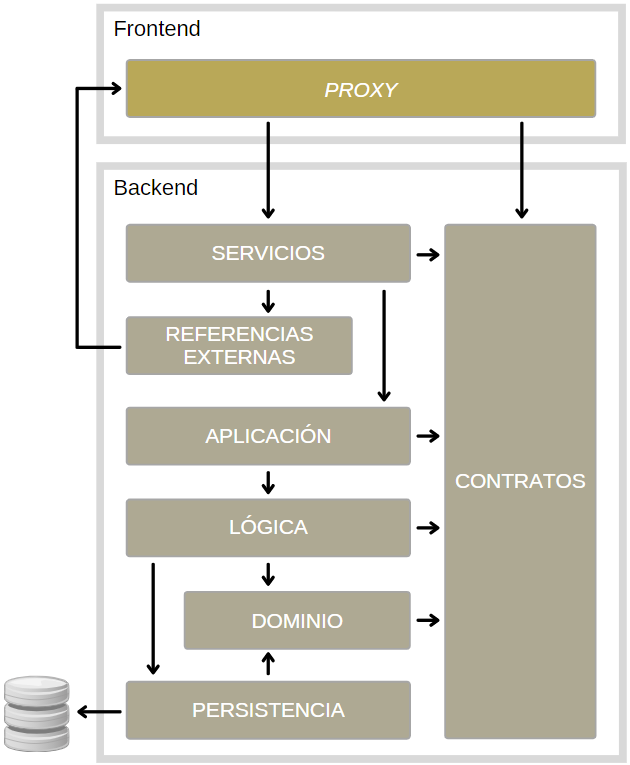
\includegraphics[width=0.55\textwidth]{imagenes/arquitectura}
\caption{Esquema de las capas de la arquitectura del \emph{proxy} inverso.}
	\label{arquitectura}
\end{figure}

			%%%%%%%%%%%%%%%%%%%%%%%%%%%%%% CAPA DE LÓGICA %%%%%%%%%%%%%%%%%%%%%%%%%%%%%%

			\subsubsection{Capa de lógica}

La capa que más ha sido necesario modificar es la de lógica, pues las acciones del \emph{proxy} inverso se implementan en ella. Es por esto que se va a entrar en más detalle acerca de esta capa. Las figuras \ref{proyectoLogica} y \ref{proyectoTestsLogica} muestran la estructura de carpetas y clases que forman los proyectos de la capa de lógica y de sus pruebas, respectivamente. No todas las clases pero sí las más importantes serán comentadas a continuación.

\begin{figure}[ht]
\centering
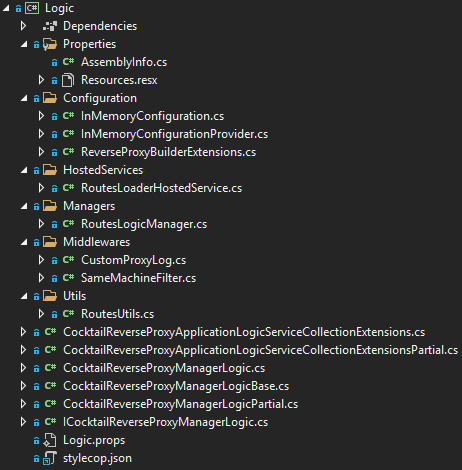
\includegraphics[width=0.8\textwidth]{imagenes/proyectoLogica}
\caption{Proyecto de Visual Studio de la capa de lógica.}
	\label{proyectoLogica}
\end{figure}

\begin{figure}[ht]
\centering
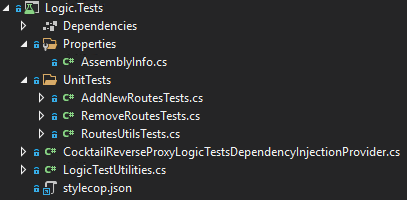
\includegraphics[width=0.7\textwidth]{imagenes/proyectoTestsLogica}
\caption{Proyecto de Visual Studio de pruebas para la capa de lógica.}
	\label{proyectoTestsLogica}
\end{figure}

En el proyecto de lógica de la figura \ref{proyectoLogica} son reseñables los siguientes aspectos:

\begin{itemize}

	\item La carpeta \emph{Configuration} contiene clases que se encargan de procesar y llevar a cabo los cambios de configuración de rutas de manera dinámica. Utilizan y se comunican con las interfaces definidas por YARP para ello.

	\item La clase \emph{RoutesLoaderHostedService} se encarga de realizar una carga inicial de rutas predefinidas, esto es, cuando se inicia el microservicio.

	\item El \emph{RoutesLogicManager} implementa las acciones propias del \emph{proxy} inverso, es decir, las acciones de añadir y eliminar rutas.

	\item La carpeta llamada \emph{Middlewares} contiene los \emph{middlewares} creados que se añaden a la \emph{pipeline} de YARP. Se profundiza en esto en el siguiente apartado, \ref{pipelineYARP}.

	\item La clase \emph{RoutesUtils} extrae métodos de ayuda que se utilizan de forma repetida tales como la creación de identificadores de manera idempotente.

\end{itemize}

En el proyecto de pruebas (figura \ref{proyectoTestsLogica}) simplemente destacar la existencia de tres clases de prueba principales: \emph{AddNewRoutesTests}, \emph{RemoveRoutesTests} y \emph{RoutesUtilsTests}. La primera es para la acción de añadir rutas, la segunda para la de eliminarlas y la tercera para la clase \emph{RoutesUtils}. Por último, la clase \emph{LogicTestUtilities} incluye funciones auxiliares para realizar comprobaciones que se repiten en más de una prueba, como por ejemplo la comprobación de si una determinada ruta existe.

		%%%%%%%%%%%%%%%%%%%%%%%%%%%%%% PIPELINE DE YARP %%%%%%%%%%%%%%%%%%%%%%%%%%%%%%

		\subsection{\emph{Pipeline} de YARP} \label{pipelineYARP}

Una \emph{pipeline} se entiende como una sucesión de procesos que se ejecutan en cadena de manera que la salida de cada uno de ellos se conecta con la entrada del siguiente. Importante destacar que, debido a esa sucesión, el orden en el que se ejecutan los diferentes procesos sí es relevante. Para gestionar las peticiones, ASP.NET define una de ellas en el método \emph{Configure} \cite{MiddlewaresPipeline}. Está formada por componentes llamados \emph{middlewares}, con un determinado propósito cada uno de ellos. Los \emph{middlewares} disponibles cubren aspectos tales como páginas de excepciones especiales para el desarrollador, control de excepciones o seguridad de transporte.

Por su parte, YARP tiene una propia, integrada en la de .NET. Por defecto, sus \emph{middlewares} se encargan de realizar sesión de afinidad para las peticiones, balanceo de carga, \emph{health checks} pasivos y el enrutamiento final. Sin embargo, se puede personalizar añadiendo nuevos \emph{middlewares} hechos desde cero según la necesidad del desarrollador. La figura \ref{pipelineYARP_imagen} muestra como ha quedado configurada esta última en el \emph{proxy} inverso. En ella, se observa que se han utilizado los siguientes:

\begin{figure}[ht]
\centering
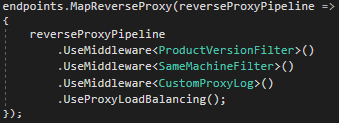
\includegraphics[width=0.6\textwidth]{imagenes/pipelineYARP}
\caption{\emph{Pipeline} de YARP configurada para el \emph{proxy} inverso.}
	\label{pipelineYARP_imagen}
\end{figure}

\begin{itemize}

	\item \textbf{\emph{ProductVersionFilter}}. Este \emph{middleware} surge de la posibilidad de coexistir más de una versión del mismo \emph{endpoint}. Así pues, es el encargado de averiguar qué versión de API quiere utilizar cada petición que se recibe para eliminar las posibles destinaciones que tengan una diferente. De esta manera, se asegura que las peticiones serán redirigidas a un \emph{endpoint} con la versión correcta. Dicha información se manda en cada petición dentro de un \emph{header} y, en caso de no encontrar ninguna destinación disponible con la versión correcta, se envía hacia el \emph{endpoint} con versión mayor.

	\item \textbf{\emph{SameMachineFilter}}. Su finalidad es filtrar las posibles destinaciones del enrutamiento de una petición de forma que si una de las direcciones corresponde a la misma máquina en la que se encuentra el \emph{proxy} inverso, sea redirigida hacía ella. Esto puede suceder cuando el microservicio destino se encuentra desplegado en la misma máquina. De esta manera se ahorra tiempo evitando hacer una petición a otra dirección.

	\item \textbf{\emph{CustomProxyLog}}. Se encarga de personalizar los mensajes de \emph{log} que muestra el \emph{proxy} inverso por consola cuando enruta una petición. YARP muestra por defecto un mensaje pero se considera interesante mostrar más información para facilitar las tareas de depuración, por ejemplo.

	\item \textbf{\emph{ProxyLoadBalancing}}. No es un \emph{middleware} creado para este proyecto, se trata de uno predefinido por YARP que se encarga de realizar las tareas de balanceo de carga cuando una misma ruta tiene diferentes posibles destinaciones. En concreto, elige una entre las disponibles en base a un algoritmo que se puede configurar. Tiene que ser el último \emph{middleware} añadido porque es él el que se encarga de elegir finalmente dónde se redirigen las peticiones de entre las destinaciones disponibles y no filtradas por los anteriores.

\end{itemize}

	%%%%%%%%%%%%%%%%%%%%%%%%%%%%%% METODOLOGÍA %%%%%%%%%%%%%%%%%%%%%%%%%%%%%%

	\section{Metodología} \label{metodologia}

Para llevar a cabo este desarrollo se ha seguido un enfoque ágil en el sentido de que se han seguido algunas de las prácticas propuestas por varias de las metodologías de este tipo, tales como Scrum o Kanban, con el fin de seguir un enfoque metodológico personalizado y adaptado a las características del proyecto. Las prácticas utilizadas se detallan a continuación:

\begin{itemize}

	\item \textbf{Organización de las tareas en unidades de trabajo}. El trabajo a realizar para construir el \emph{proxy} inverso se ha divido en tareas menudas denominadas unidades de trabajo. Estas definen funcionalidades más pequeñas y concretas que los casos de uso y son más abstractas que las historias de usuario, ya que manifiestan de forma más clara la posibilidad de tratarse de tareas no solo relacionadas con cambiar el producto sino otras como crear una base de datos o renovar una suscripción de un servicio web.

	\item \textbf{Uso de un tablero \emph{kanban}}. En relación con la anterior práctica ágil, las unidades de trabajo han sido gestionadas a través de un tablero \emph{kanban} con tres columnas: \emph{TODO}, \emph{DOING}, \emph{DONE}. La única columna reseñable es la segunda, en la que primero se lleva a cabo una pequeña especificación de la unidad de trabajo en cuestión, principalmente definiendo sus pruebas de aceptación, y después, se implementa. Cabe destacar que el tablero utilizado es muy simple, sin embargo, podía haberse tratado de uno más complejo si el desarrollo se hubiera llevado a cabo en equipo con más personas. La herramienta utilizada a modo de tablero \emph{kanban} ha sido Trello \footnote{Web oficial de Trello: \url{https://trello.com}.}.

	\item \textbf{Priorización de las unidades de trabajo}. Dentro de la propia columna \emph{TODO} del tablero \emph{kanban}, las unidades de trabajo han estado ordenadas de mayor a menor importancia en todo momento. Este almacén de trabajo priorizado a realizar se conoce como \emph{backlog} y ha permitido conocer con facilidad las unidades de trabajo que se debían abordar al terminar otras.

	\item \textbf{Definición de pruebas de aceptación}. Se ha utilizado este tipo de pruebas para especificar las unidades de trabajo correspondientes a la funcionalidad básica del \emph{proxy} inverso. Con ellas se establecen los límites de lo que se ha de considerar funcionamiento correcto o incorrecto. Además, algunas de las pruebas de aceptación han sido automatizadas, es decir, programadas dentro del propio proyecto, sistematizando y haciendo más fácil su ejecución. Se entrará más en detalle sobre las pruebas de aceptación definidas en el apartado \ref{pruebasDeAceptacion}.

	\item \textbf{Búsqueda de la sencillez y el minimalismo}. Se trata de no realizar esfuerzos innecesarios a la hora de implementar una determinada funcionalidad, esto es, buscar la solución más simple que cumpla los requisitos establecidos. De esta forma, se evita invertir tiempo en aspectos no definitivos o que se modificarán con posterioridad y que no afectan al funcionamiento inmediato del producto.

	\item \textbf{Afrontamiento y entrega de trabajo terminado de forma incremental}. Con el uso de unidades de trabajo se ha pretendido dividir y afrontar el trabajo a realizar mediante incrementos de funcionalidad, definidos precisamente por un conjunto de unidades de trabajo. Además, a medida que se ha terminado cada uno de estos incrementos, se ha entregado una nueva versión del producto. En este caso, las entregas del producto han correspondido con el despliegue de la determinada versión, quedando disponible para ser utilizada por el resto de la aplicación.

	\item \textbf{Ejecución de pruebas de regresión}. Han consistido en ejecutar las pruebas de aceptación de todas las unidades de trabajo finalizadas hasta la fecha cada vez que un incremento considerable de funcionalidad era terminado. Con estas se consigue asegurar el correcto funcionamiento del producto antes de cada nueva entrega o despliegue. Las pruebas de regresión llevadas a cabo en este proyecto se comentarán en el apartado \ref{pruebasDeRegresion}.

\end{itemize}

		%%%%%%%%%%%%%%%%%%%%%%%%%%%%%% PLAN DE TRABAJO %%%%%%%%%%%%%%%%%%%%%%%%%%%%%%

		\subsection{Plan de trabajo} \label{planDeTrabajo}

Tras la exposición de la metodología seguida para este proyecto, se va a detallar el plan de trabajo trazado. La elaboración del tablero \emph{kanban} se ha tomado como punto de partida y se muestran sus unidades de trabajo iniciales en la figura \ref{kanbanInicial}, las cuales fueron obtenidas a partir de la especificación de requisitos del apartado \ref{especificacionRequisitos}. Cabe destacar que estas no han sido las definitivas y posteriormente se han modificado y creado nuevas, como es habitual en las metodologías ágiles.

\begin{figure}[ht]
\centering
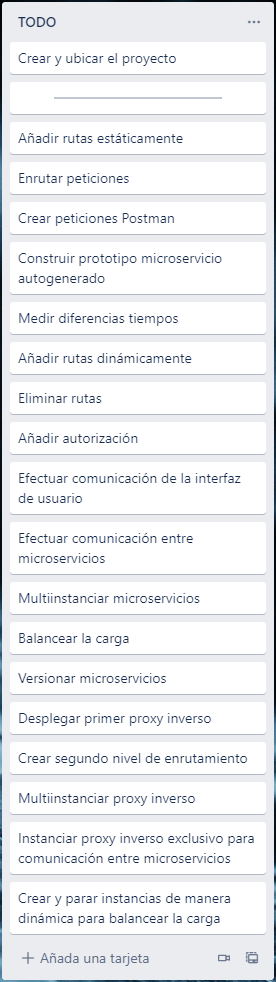
\includegraphics[width=0.34\textwidth]{imagenes/backlogInicial}
\caption{\emph{Backlog} con las unidades de trabajo iniciales.}
	\label{kanbanInicial}
\end{figure}

Una vez elaborado y priorizado el \emph{backlog}, el plan de trabajo ha sido hacer uso del tablero \emph{kanban} e ir desarrollando incrementos de funcionalidad poniendo en práctica las características ágiles comentadas en el punto anterior.

Por último, es interesante comentar el inicio particular de este desarrollo, pues se planificó la elaboración de dos prototipos de microservicio. Estos tendrían la misión de demostrar si el uso de código autogenerado a partir de modelos, como en el resto de microservicios, penaliza en exceso el rendimiento del \emph{proxy} inverso. Esto podía deberse al tratarse de un código menos específico y más genérico, así como al poseer un exceso de características innecesarias para el caso en cuestión pero que sí son adecuadas para el resto de microservicios.

Así pues, la construcción de los prototipos culminaría en una medición de tiempos para evaluar la eficiencia de las dos soluciones y la consiguiente elección para continuar con el desarrollo de uno u otro prototipo. Se ahondará en todo este proceso en el siguiente apartado.

TODO: Faltaría añadir Cronología del proyecto: hitos principales (apartado 4.4, estudio de tecnologías, revisión de memoria).

	%%%%%%%%%%%%%%%%%%%%%%%%%%%%%% PROGRAMACIÓN %%%%%%%%%%%%%%%%%%%%%%%%%%%%%%

	\section{Programación} \label{programacion}

La parte de programación del \emph{proxy} inverso que protagoniza este trabajo ha pasado por distintas etapas o fases que se van a comentar a continuación. Estas etapas han sido creadas para facilitar la comprensión del desarrollo y las funcionalidades añadidas al producto. De esta forma, las agrupan para comentarlas poco a poco junto con los problemas o dificultades encontradas a la hora de implementarlas.

		%%%%%%%%%%%%%%%%%%%%%%%%%%%%%% CONSTRUCCIÓN DE PROTOTIPOS %%%%%%%%%%%%%%%%%%%%%%%%%%%%%%

		\subsection{Construcción de prototipos}

Como el plan de trabajo del punto \ref{planDeTrabajo} establece, el desarrollo comienza con la elaboración de dos prototipos de microservicio para evaluar la viabilidad de utilizar la estructura autogenerada de los demás microservicios sobre el \emph{proxy} inverso. De esta forma, se construyó un microservicio sin utilizar la generación de código y otro utilizándola para medir posteriormente las diferencias de rendimiento entre uno y otro. Por otro lado, cabe destacar que a los \emph{proxy} inversos que forman parte de una arquitectura de microservicios no se les suele dar tal categoría. Sin embargo, en este trabajo sí se le va a incluir dentro de los denominados microservicios debido a que se quiere que tenga la misma estructura, RNF04 del apartado \ref{requisitosNoFuncionales}. Al fin y al cabo es un tema simplemente de nomenclatura.

			%%%%%%%%%%%%%%%%%%%%%%%%%%%%%% MICROSERVICIO A MANO %%%%%%%%%%%%%%%%%%%%%%%%%%%%%%

			\subsubsection{Microservicio a mano}

El primero de los prototipos se hizo lo más simple posible, es decir, con la lógica justa y necesaria para desempeñar su trabajo y sin seguir ninguna arquitectura concreta. Esto último choca con el requisito no funcional comentado en el párrafo anterior pero se hizo para que las diferencias de rendimiento se evidenciaran más todavía, pues así se compararía un prototipo únicamente con el funcionamiento de \emph{proxy} inverso y otro con también una estructura con multitud de clases que pudiera penalizar el rendimiento.

Para la creación de este prototipo, primero fue necesario crear un proyecto desde cero y ubicarlo en el lugar correspondiente del directorio de carpetas de la aplicación, junto a los demás microservicios. Acto seguido, se añadió el funcionamiento de \emph{proxy} inverso dado por YARP (CU03 del apartado \ref{casosDeUso}) y se le crearon rutas de manera predefinida para hacer las primeras pruebas con peticiones Postman. Las rutas predefinidas se configuran en el archivo \emph{appsettings.json}. Estos dos últimos aspectos se comentan con más detalle en el apartado \ref{ejemploUsoYARP} y un ejemplo de configuración de rutas estáticas se puede ver en la figura \ref{ejemploYARP_appsettings}.

Después de realizar las tareas comentadas queda un proyecto muy simple pero totalmente funcional. Se muestra la solución de Visual Studio correspondiente en la figura \ref{prototipoMano}.

\begin{figure}[ht]
\centering
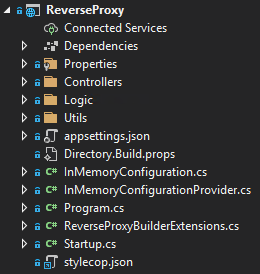
\includegraphics[width=0.5\textwidth]{imagenes/prototipoMano}
\caption{Solución de Visual Studio del prototipo de \emph{proxy} inverso hecho a mano.}
	\label{prototipoMano}
\end{figure}

			%%%%%%%%%%%%%%%%%%%%%%%%%%%%%% MICROSERVICIO AUTOGENERADO %%%%%%%%%%%%%%%%%%%%%%%%%%%%%%

			\subsubsection{Microservicio autogenerado}

Respecto al segundo prototipo, fue construido utilizando las mismas herramientas de generación automática de código con las que fueron construidos el resto de microservicios de la aplicación. Cabe destacar que, para no realizar esfuerzos en vano (práctica ágil comentada en el apartado \ref{metodologia}) sin saber qué prototipo iba a ser la opción elegida, se dejaron algunos detalles correspondientes a la generación de código pendientes. Esto se debe a que el proceso de generación de código no se adaptaba al cien por cien a las necesidades del nuevo microservicio, lo que suele ser habitual al crear microservicios con características diferentes.

Así pues, se creó desde cero otro proyecto, ahora utilizando la generación automática de código a partir de modelos. Para ello fue necesario modelar una entidad \emph{Route} con los campos necesarios para identificar las rutas, esto es, la ruta base de las peticiones que se tiene que capturar y la dirección a la que redirigirlas. También se escribió el código correspondiente a YARP para crear el \emph{proxy} inverso y se configuraron algunas rutas por defecto. Por último, se crearon algunas consultas Postman para probar este prototipo. Estas tres últimas acciones son las mismas que para el caso del microservicio manual, con algunas diferencias para adaptarse a la solución concreta.

El microservicio autogenerado resultante se muestra en la figura \ref{prototipoAutogenerado}. Es interesante comparar esta solución con la del prototipo hecho a mano para comprobar que la complejidad y cantidad de proyectos de Visual Studio, y por consiguiente también de clases, es muchísimo mayor en este caso. Cabe resaltar que faltarían los proyectos correspondientes a la capa de dominio y contratos, los cuales se encuentran en una solución aparte y no es necesario mostrarlos para realizar esta comparativa puesto que las evidencias comentadas son suficientes.

\begin{figure}[ht]
\centering
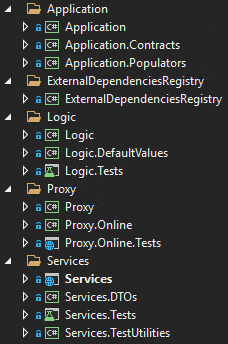
\includegraphics[width=0.45\textwidth]{imagenes/prototipoAutogenerado}
\caption{Solución de Visual Studio del prototipo de \emph{proxy} inverso hecho con generación de código.}
	\label{prototipoAutogenerado}
\end{figure}

			%%%%%%%%%%%%%%%%%%%%%%%%%%%%%% COMPARATIVA %%%%%%%%%%%%%%%%%%%%%%%%%%%%%%

			\subsubsection{Comparativa}

Una vez construidos los prototipos, se procedió a medir el impacto de seguir la norma para decidir qué prototipo desechar y con cuál seguir adelante. Para ello, se creó una aplicación de consola muy simple que se encargara de probar los dos microservicios de \emph{proxy} inverso creados. Esta lanzaba un número determinado de veces la misma petición sobre el \emph{proxy} inverso que se le indicara para que este la redirigiera y calcular así el tiempo medio de respuesta. La figura \ref{medidorTiempos} muestra su código principal, el cual era ejecutado una vez por cada prototipo.

\begin{figure}[ht]
\centering
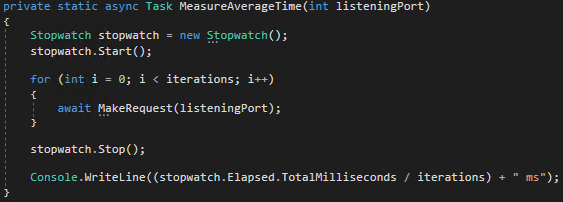
\includegraphics[scale=1]{imagenes/medidorTiempos}
\caption{Código principal de la aplicación de consola para medir los tiempos del enrutamiento de los dos prototipos.}
	\label{medidorTiempos}
\end{figure}

Es importante destacar que las acciones de añadir y eliminar rutas dinámicamente, todavía por implementar, no son relevantes en esta comparativa ya que se llevan a cabo muy pocas veces en relación con el enrutamiento, es decir, no son las más comunes. Por este motivo, no se ha creído conveniente medirlas y han sido implementadas con posterioridad.

Por otro lado, es interesante comentar por qué desde un primer momento se enfocaba la comparativa como una prueba para ver si el microservicio autogenerado era viable y, por tanto, preferible sobre el otro. Uno de los motivos era que, si se utilizaba la generación de código, el \emph{proxy} inverso se podría desplegar con el mismo procedimiento que estaba pensado para el resto de microservicios, lo que evitaría tener que crear un mecanismo especial para él y permitiría conservar esa homogeneidad para simplificar los despliegues. Otro motivo se trataba de la trivialidad para hacer cualquier cambio de estructura, pues la generación de código lo haría de forma automática. Por el contrario, habría que hacerlo manualmente en el microservicio a mano para continuar con el cumplimiento del requisito no funcional RNF04, del apartado \ref{requisitosNoFuncionales}.

Los resultados de las mediciones fueron claros: ambos prototipos tenían un rendimiento casi idéntico.
En concreto, para 10000 iteraciones se obtuvieron tiempos medios de respuesta de 3,6 milisegundos para el prototipo a mano y de 3,7 para el autogenerado. Se realizaron pruebas con diferente número de iteraciones pero los resultados no variaron en demasía. Con esto se concluye que utilizar el segundo prototipo supone una penalización de tiempo de no llega al 3\%. Esto se consideró despreciable e insuficiente para contrarrestar las ventajas comentadas por lo que se decidió eliminar el primer prototipo y continuar así con la versión autogenerada.

		%%%%%%%%%%%%%%%%%%%%%%%%%%%%%% CONSOLIDACIÓN DEL MICROSERVICIO AUTOGENERADO %%%%%%%%%%%%%%%%%%%%%%%%%%%%%%

		\subsection{Consolidación del microservicio autogenerado}

Una vez elegida la opción de seguir el estándar de microservicio de la aplicación, hubo que resolver los aspectos de la generación de código que no quedaron ajustados. Así pues, se tuvieron que modificar algunas plantillas de código a partir de las cuales se generan las clases y proyectos que forman los microservicios.

Un ejemplo de problemas con la generación de código fue el método \emph{Configure} de la clase \emph{Startup}. Este tenía que ser modificado para añadir la llamada \emph{endpoint.MapReverseProxy()} pero la generación de código no lo permitía, no pudiéndose personalizar este método en función del microservicio en cuestión. De esta forma, la modificación de las plantillas consistió en generar una llamada a un método estático dentro de ese \emph{Configure}, que se implementaría en una clase parcial. La figura \ref{startup} muestra cómo queda la clase \emph{Startup}.

\begin{figure}[ht]
\centering
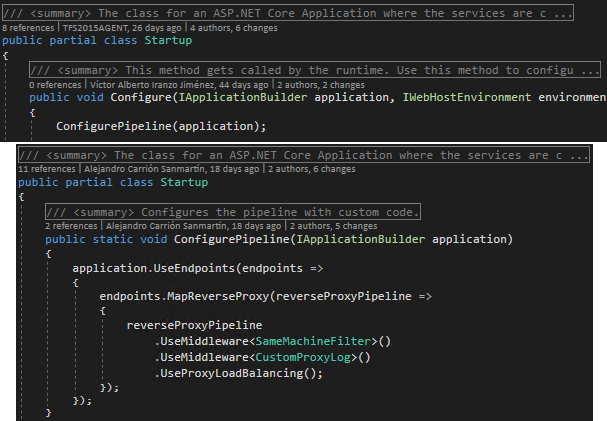
\includegraphics[width=1\textwidth]{imagenes/startup}
\caption{Clase parcial \emph{Startup} del \emph{proxy} inverso.}
	\label{startup}
\end{figure}

Después de terminar los flecos de generación de código, era momento de seguir añadiendo funcionalidad. De este modo, se modelaron e implementaron las acciones de añadir y eliminar rutas dinámicamente, correspondientes a los casos de uso CU01 y CU02 del apartado \ref{casosDeUso}. También fueron probadas con las correspondientes peticiones Postman.

Por otro lado, se añadió un mecanismo de autenticación de peticiones, tal y como demanda el requisito no funcional RNF01 de la sección \ref{requisitosNoFuncionales}. Este consistió simplemente en utilizar el mismo mecanismo de seguridad que se utiliza en el resto de microservicios, el cual utiliza el sistema de autenticación que ofrece .NET y se genera de manera automática para las acciones modeladas, como es el caso de las dos acciones comentadas en el párrafo anterior. Solo sería necesario indicar a YARP que utilizase dicho mecanismo también a la hora de enrutar peticiones.

También se creyó conveniente estandarizar el tratamiento de las rutas base de las peticiones que representan una ruta. Esto se hizo para hacer el \emph{proxy} inverso más robusto y evitar posibles malentendidos con YARP, pues espera recibir las rutas de una manera concreta y no otra. Por ejemplo, requiere que se utilicen barras como separadores de ruta en lugar de barras invertidas. Para ello se creó un método \emph{GetYarpNormalizedPath}, en la clase \emph{RoutesUtils}, que normaliza una ruta dada según el esquema que YARP acepta. El método en cuestión se muestra en la figura \ref{getYarpNormalizedPath} y hace cosas como forzar el uso de las barras como separadores o añadir el patrón ''\emph{\{*remainder\}}'' para capturar todas las peticiones con rutas que empiecen con el prefijo indicado independientemente de como sigan.

\begin{figure}[ht]
\centering
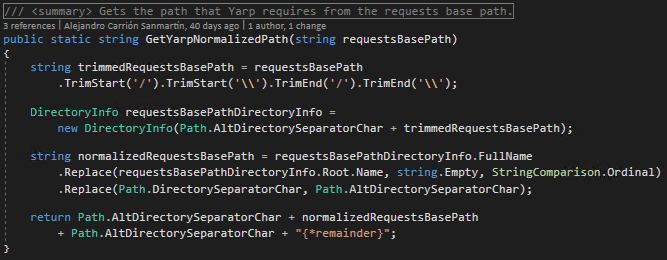
\includegraphics[width=1\textwidth]{imagenes/getYarpNormalizedPath}
\caption{Método \emph{GetYarpNormalizedPath}.}
	\label{getYarpNormalizedPath}
\end{figure}

Además, se consideró oportuno automatizar algunas de las pruebas de aceptación de las acciones de añadir y eliminar rutas y para el método \emph{GetYarpNormalizedPath}, recién comentado en el párrafo anterior. Se entrará más en detalle acerca de estas pruebas en el apartado de pruebas \ref{pruebas}.

Por último, se incluyó el \emph{proxy} inverso en el núcleo de microservicios principales llamados Core. Estos son los que se despliegan en primer lugar ya que son utilizados por todos los demás, o al menos por la mayoría. Se ahondará en este aspecto de los despliegues en el siguiente apartado. Microservicios de este tipo son los que se encargan de aspectos clave tales como la seguridad, el despliegue de la aplicación o, como es el caso de este, la comunicación entre los microservicios.

		%%%%%%%%%%%%%%%%%%%%%%%%%%%%%% PRIMEROS DESPLIEGUES %%%%%%%%%%%%%%%%%%%%%%%%%%%%%%

		\subsection{Primeros despliegues}

A estas alturas del desarrollo ya se tenía una primera versión del \emph{proxy} inverso perfectamente funcional pero antes de llevar a cabo los primeros despliegues había que hacer algunas modificaciones para que la interfaz de usuario y los microservicios lo utilizaran. Derivado de estos despliegues se presentaron algunos problemas que también serán comentados.

			%%%%%%%%%%%%%%%%%%%%%%%%%%%%%% SISTEMAS DE DESPLIEGUE %%%%%%%%%%%%%%%%%%%%%%%%%%%%%%

			\subsubsection{Sistema de despliegue}

Primero de todo, se va a explicar como se realizan los despliegues de la aplicación. Como se ha comentado de pasada en varios puntos de esta memoria, la aplicación sobre la cual se trabaja tiene un microservicio especial encargado de orquestar los despliegues. La cuestión es que no está del todo operativo todavía, pues la aplicación se encuentra en desarrollo, y por este motivo se realizan dos tipos de despliegue:

\begin{itemize}

	\item El primero de ellos consiste en desplegar los microservicios mediante contenedores Docker \footnote{Web oficial de Docker: \url{https://www.docker.com}.}. Se trata de una manera de poder realizar despliegues antes de que el microservicio específico esté terminado. Permite así hacer pruebas con el resto y ver como se comportan.

	\item El segundo es el que lleva a cabo el microservicio pensado para ello. A grandes rasgos, este ordena y organiza los servidores preparados para correr la aplicación y les dice a cada uno qué microservicio o microservicios tiene que ejecutar. Por el momento, los microservicios que despliega no se utilizan porque se encuentra en fase de pruebas.

\end{itemize}

Una vez expuestos los modos de despliegue y el por qué de su coexistencia, cabe resaltar que el \emph{proxy} inverso se ve obligado a ser capaz de trabajar con ambos. No obstante, en un futuro desaparecerá el primero de ellos y el segundo será el que se emplee de manera definitiva.

			%%%%%%%%%%%%%%%%%%%%%%%%%%%%%% INTERFAZ DE USUARIO %%%%%%%%%%%%%%%%%%%%%%%%%%%%%%

			\subsubsection{Interfaz de usuario}

Para empezar con los despliegues, se decidió hacer que solo la interfaz de usuario utilizara el \emph{proxy} inverso para no romper toda la aplicación en caso de fallar. Cabe destacar que, como la aplicación se encontraba todavía en fase de desarrollo, no hubiera sido un gran problema si la interfaz de usuario quedara inutilizable por un breve periodo de tiempo por culpa del nuevo microservicio. Sin embargo, la caída del \emph{backend} podría haber supuesto algún inconveniente para el resto del equipo de la aplicación puesto que no sería posible hacer pruebas sobre los microservicios desplegados. De esta manera, se pretendía minimizar riesgos.

Además, como paso previo a incluir el \emph{proxy} inverso al proceso de despliegue, también se hicieron pruebas de manera local para comprobar que todo funcionaba correctamente y que la interfaz de usuario no se iba a quedar caída. Se desplegó el \emph{proxy} inverso en una máquina a parte y se le cargó de rutas que apuntaban a los microservicios ya desplegados para que la interfaz de usuario lo utilizara. Se hicieron peticiones desde dicha interfaz de usuario y no hubo problemas.

La interfaz de usuario de la aplicación se conectaba directamente a los microservicios por lo que hizo falta interponer el nuevo componente entre ella y el \emph{backend}. Para ello, fue necesario modificar las direcciones a las que apuntaba, en concreto, substituir las de cada microservicio por la del \emph{proxy} inverso. De esta forma, la interfaz de usuario dejaba de conocer todos los microservicios para solo conocer su dirección.

No obstante, las direcciones de los microservicios ahora debían ser conocidas por el \emph{proxy} inverso, por lo que hubo que cargárselas. Aquí es donde entran en juego los diferentes modos de despliegue. Para los despliegues con el microservicio específico, esté es quien tiene que cargar de rutas el \emph{proxy} inverso cada vez que le ordene a un servidor ejecutar un determinado microservicio. Con respecto al despliegue en Docker, las rutas han de ser cargadas de una manera predefinida. Para especificar dichas rutas, se ha creado un fichero llamado \emph{defaultRoutes.json} (figura \ref{defaultRoutes}), que es leído al iniciarse el \emph{proxy} inverso y las rutas que describe son añadidas.

\begin{figure}[ht]
\centering
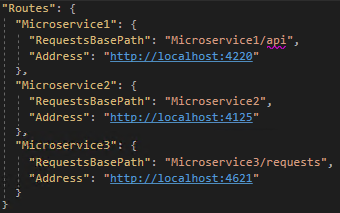
\includegraphics[width=0.6\textwidth]{imagenes/defaultRoutes}
\caption{Fichero \emph{defaultRoutes.json}.}
	\label{defaultRoutes}
\end{figure}

			%%%%%%%%%%%%%%%%%%%%%%%%%%%%%% MICROSERVICIOS %%%%%%%%%%%%%%%%%%%%%%%%%%%%%%

			\subsubsection{Microservicios}

Una vez la interfaz de usuario funcionaba correctamente con el \emph{proxy} inverso desplegado, se hizo que los propios microservicios lo utilizaran para comunicarse entre ellos. Igual que en el caso anterior, también fue necesario cambiar las direcciones a las que apuntaban los microservicios, ahora pasarían a conocer solo al \emph{proxy} inverso.

Por otro lado, una vez más hay que diferenciar los cambios para los dos modos de despliegue. Al respecto del de Docker, también se añadieron al \emph{defaultRoutes.json} las rutas que fueron necesarias, correspondientes a algunos microservicios que no son utilizados por la interfaz de usuario. En referencia al segundo, se mejoró la manera en la que el microservicio de despliegue añadía rutas al \emph{proxy} inverso.

Como modificación común para los dos modos, se tuvo que repensar el orden de despliegue de los microservicios. Estos, cuando son levantados, intentan contactar con sus dependencias y fallan si no las encuentran vivas. Por este motivo, el \emph{proxy} inverso debe estar en marcha cuando esta especie de saludos se lleven a cabo. El problema es que él también depende de otros microservicios, creando así un círculo de dependencias. La solución por la que se apostó fue levantar a la vez los microservicios que se entrelazan en este círculo utilizando reintentos en todas sus llamadas.

			%%%%%%%%%%%%%%%%%%%%%%%%%%%%%% PROBLEMAS %%%%%%%%%%%%%%%%%%%%%%%%%%%%%%

			\subsubsection{Problemas}

El problema más grande que surgió a raíz de los primeros despliegues fue con unos \emph{timeouts}. Resulta que dos microservicios concretos realizaban determinadas peticiones con un \emph{timeout} muy grande debido al elevado coste de las mismas y por algún motivo dichas peticiones no se completaban satisfactoriamente al pasar por el \emph{proxy} inverso. El código de estado de error que tenían era el 504, correspondiente al mensaje en inglés ''\emph{Gateway timeout}''. Parecía que el \emph{proxy} inverso cortaba las llamadas antes de que terminaran. Para solucionarlo momentáneamente y no dejar caídos esos microservicios, se optó por hacer que ellos y solo ellos no lo utilizaran hasta que el problema fuera analizado en detalle.

El problema recién expuesto fue estudiado a fondo más tarde y al final resultó ser culpa de YARP, que utiliza un timeout por defecto de 100 segundos para redirigir peticiones. La solución fue aumentarlo para las rutas correspondientes a las peticiones que se redirigen hacia los microservicios en cuestión. Para ello, fue necesario modelar y añadir un parámetro opcional para el \emph{timeout} en la creación de las rutas. De esta forma se permite su personalización en función de la ruta que se utilice.

La solución dada al problema puede parecer que no es la óptima ya que cualquier petición relacionada con una ruta de \emph{timeout} grande podría durar más de lo esperado, es decir, el aumento del \emph{timeout} afecta a todas las peticiones que se emparejan con esa ruta, siendo no del todo correcto. Una posible mejora sería crear rutas específicas con \emph{timeouts} grandes para solo las peticiones que lo necesiten. No obstante, no se cree necesario complicar el funcionamiento de esa manera ya que, en la práctica, el comportamiento del \emph{proxy} inverso no variaría demasiado. Además, si un cliente con un determinado \emph{timeout} realiza una petición a través del \emph{proxy} inverso y la ruta correspondiente tiene uno mayor, el que prevalecerá será el del cliente y el del \emph{proxy} inverso no tendrá efecto. De esta manera, solo sirve de límite en caso de que el del \emph{proxy} inverso sea menor.

Un problema menor que también surgió fue uno relacionado con los códigos de estado de las peticiones. El \emph{proxy} inverso devolvía uno con número 502. Este a menudo era confundido con el 504 recién explicado y provocaba malentendidos. Su mensaje en inglés era ''\emph{Bad Gateway}'', lo que parecía ser culpa del nuevo componente, generando confusión en el resto de desarrolladores de la aplicación. Finalmente resultó ser debido a enrutamientos cuyo destino no estaba disponible, es decir, el \emph{proxy} inverso no tenía ninguna culpa, simplemente mostraba un 502 en lugar del habitual 404, ''\emph{Not Found}'', que se hubiera mostrado en caso de que las peticiones no fueran respuestas por su destinatario.

		%%%%%%%%%%%%%%%%%%%%%%%%%%%%%% PRODUCTO FINAL %%%%%%%%%%%%%%%%%%%%%%%%%%%%%%

		\subsection{Producto final}

En esta etapa final se hicieron algunos retoques y se implementaron algunas funcionalidades más que se pasan a detallar.

			%%%%%%%%%%%%%%%%%%%%%%%%%%%%%% PERSONALIZACIÓN DE LOS MENSAJES DE LOG %%%%%%%%%%%%%%%%%%%%%%%%%%%%%%

			\subsubsection{Personalización de los mensajes de log}

Una de las mejoras que se llevó a cabo fue personalizar los mensajes de \emph{log} para mostrar más información acerca de las peticiones enrutadas. YARP ya muestra mensajes pero se consideraba interesante añadir la fecha y hora en la que se produjo y el código de estado resultante de la petición. De esta manera, se facilitaría la labor de encontrar posibles errores derivados del enrutamiento de peticiones tales como el de los \emph{timeouts}. Para ello, fue necesario crear y añadir un \emph{middleware} nuevo a la \emph{pipeline} de YARP, explicada en el apartado \ref{pipelineYARP}. El \emph{middleware} creado ha sido llamado \emph{CustomProxyLog} y la figura \ref{logs} muestra los mensajes por defecto de YARP y los personalizados a través de este \emph{middleware} para ver las diferencias y el resultado final.

\begin{figure}[ht]
\centering
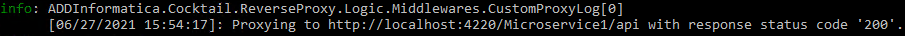
\includegraphics[width=1\textwidth]{imagenes/logs}
\caption{Mensajes de \emph{log} por defecto de YARP y personalizados.}
	\label{logs}
\end{figure}

			%%%%%%%%%%%%%%%%%%%%%%%%%%%%%% MULTIINSTANCIA DE MICROSERVICIOS %%%%%%%%%%%%%%%%%%%%%%%%%%%%%%

			\subsubsection{Multiinstancia de microservicios}

Una de las funcionalidades más importantes añadidas en esta etapa ha sido permitir la multiinstancia de microservicios. Esta consiste en soportar la coexistencia de varias instancias de un mismo microservicio de forma que las mismas peticiones puedan ser enrutadas a diferentes direcciones. De esta forma se permite tener más de un recurso atendiendo determinadas peticiones, si se necesita. Relacionado con esto, se permite también realizar balanceo de carga entre las diferentes instancias de un mismo microservicio.

Para llevar a cabo esta modificación fue necesario primero mejorar el sistema de creación de identificadores. YARP utiliza tres entidades para configurar rutas: \emph{Route}, \emph{Cluster} y \emph{Destination}. No es relevante entrar en mucho más detalle del funcionamiento interno pero sí comentar que las entidades de estos tipos necesitan un identificador único. Este se construía cuando se añadían rutas y de manera un poco rudimentaria por lo que hubo que hacer algo al respecto. La solución fue sistematizar su creación utilizando los parámetros de entrada y asegurando que no se pudieran repetir. Además, era importante que la forma de crearlos fuera idempotente, es decir, que siempre se obtuviera el mismo resultado para los mismos parámetros de entrada. Los métodos encargados de esto se encuentran en la clase \emph{RoutesUtils} y se muestran en la figura \ref{creacionIdentificadores}.

\begin{figure}[ht]
\centering
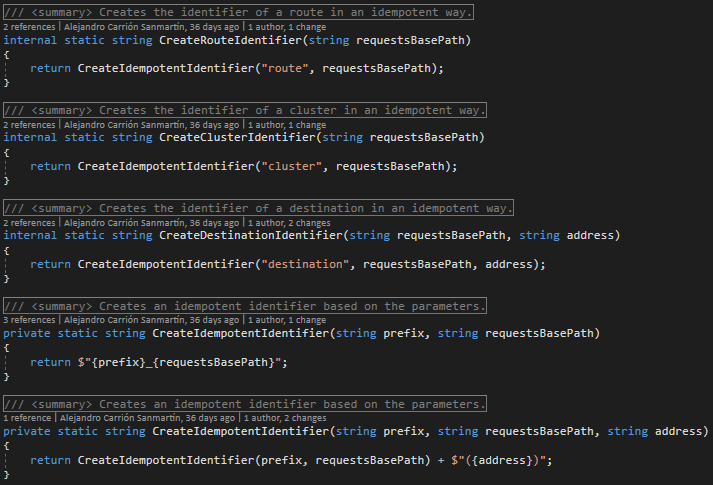
\includegraphics[width=1\textwidth]{imagenes/creacionIdentificadores}
\caption{Métodos encargados de crear los identificadores de las entidades de YARP.}
	\label{creacionIdentificadores}
\end{figure}

De una manera similar, las acciones de añadir y eliminar rutas fueron modificadas para jugar con los tres tipos de entidades de YARP. Un ejemplo del tratamiento que requieren puede ser el hecho de que un \emph{Cluster} tiene una o más \emph{Destinations}, por lo que no tendrá que ser creado si ya existe cuando se añade una nueva destinación. Todo esto sería trivial si se utilizara el mecanismo de carga estático pero, como se ha comentado en varias ocasiones a lo largo de este memoria, no encaja con el contexto de este \emph{proxy} inverso.

Por otro lado, YARP ofrece diferentes algoritmos de balanceo de carga: \emph{First}, \emph{Random}, \emph{RoundRobin}, \emph{LeastRequests} y \emph{PowerOfTwoChoices}. Se ha utilizado el último de ellos, el cual selecciona dos destinaciones aleatorias y elige la que menos peticiones esté atendiendo. Esta política intenta evitar la sobrecarga de buscar la dirección que está atendiendo menos peticiones y el caso peor de elegir de manera aleatoria una que esté muy ocupada.

Por último, las peticiones Postman se modificaron para hacer pruebas, así como las pruebas de aceptación automatizadas tuvieron que ser adaptadas e incluso se crearon algunas nuevas.

			%%%%%%%%%%%%%%%%%%%%%%%%%%%%%% SEGUNDO NIVEL DE REDIRECCIÓN %%%%%%%%%%%%%%%%%%%%%%%%%%%%%%

			\subsubsection{Segundo nivel de redirección}

Otra funcionalidad de peso es el segundo nivel de redirección. Se trata de tener un \emph{proxy} inverso en cada servidor que ejecuta alguna parte de la aplicación con la motivación de no exponer un puerto por cada microservicio. De esta forma, todas las peticiones se mandan al \emph{proxy} inverso del servidor en cuestión y este las redirige a los microservicios que corre. Esto desemboca en un esquema de dos niveles como el que se muestra en la figura \ref{esquemaProxyInversoDoble}, en el que entran en juego un \emph{proxy} inverso general y los concretos de cada servidor.

\begin{figure}[ht]
\centering
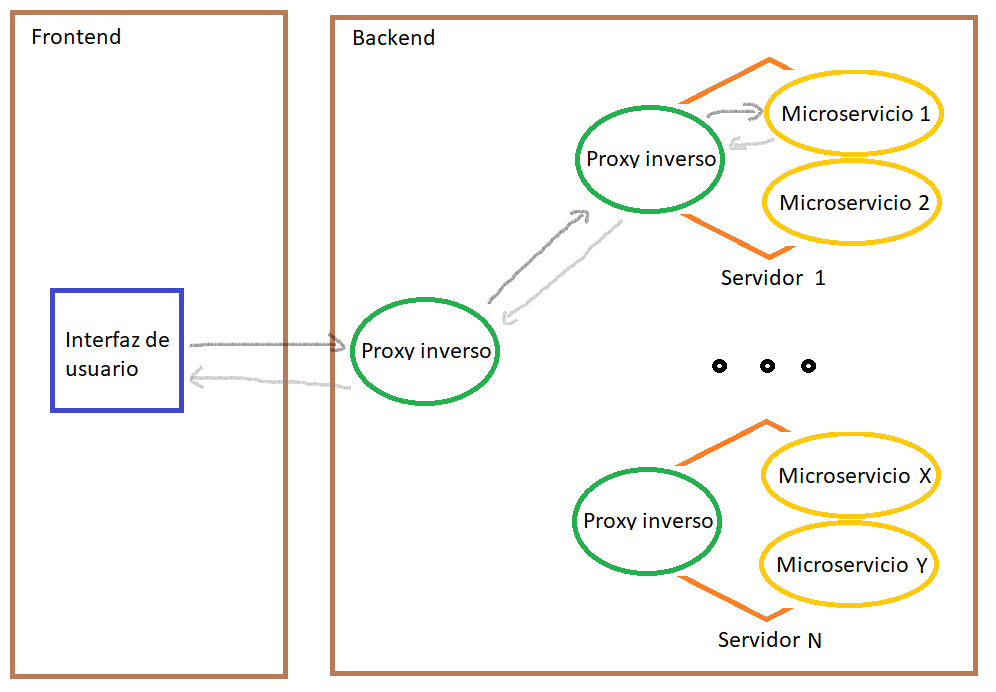
\includegraphics[width=0.9\textwidth]{imagenes/esquemaProxyInversoDoble}
\caption{Esquema de dos niveles de \emph{proxy} inverso.}
	\label{esquemaProxyInversoDoble}
\end{figure}

Para implementar esta característica se plantearon varias opciones. Primero se decidió utilizar YARP también en el código de los servidores que ejecutan los microservicios pero, al poco tiempo de empezar, se encontraron problemas y aspectos que no terminaban de cuadrar con lo que se buscaba. El más importante de ellos era el hecho de tener que mantener el código que envuelve la infraestructura de YARP en dos lugares diferentes. Para evitarlo, finalmente se optó por hacer que cada servidor ejecutara un \emph{proxy} inverso como si se tratara de un microservicio más. Es momento entonces de darse cuenta de que la elección del prototipo autogenerado fue la correcta, pues ahora permite realizar esto de una manera sencilla. También fue necesario modificar el código que carga el \emph{proxy} inverso de rutas para hacer lo propio con todos los \emph{proxy} inversos.

			%%%%%%%%%%%%%%%%%%%%%%%%%%%%%% FILTRO MISMA MÁQUINA %%%%%%%%%%%%%%%%%%%%%%%%%%%%%%

			\subsubsection{Filtro misma máquina}

Otro \emph{middleware} creado es el llamado \emph{SameMachineFilter}. Surge de las dos nuevas funcionalidades anteriores y trata de mejorar el sistema de enrutamiento disminuyendo el tiempo de algunas peticiones. Se encarga de comprobar si existe una destinación a la que redirigir las peticiones en la misma máquina que se encuentra el \emph{proxy} inverso y, si es el caso, enrutarlas hacia ella en lugar de hacia otra para evitar que la petición salga de la máquina y tarde más tiempo en finalizar.

			%%%%%%%%%%%%%%%%%%%%%%%%%%%%%% FILTRO VERSIÓN DE API %%%%%%%%%%%%%%%%%%%%%%%%%%%%%%

			\subsubsection{Filtro versión de API}

El último \emph{middleware} desarrollado es el \emph{ProductVersionFilter}. Este nombre lo recibe por aspectos concretos del sistema de despliegue que no vienen al caso. Su función es filtrar las destinaciones posibles a las que se puede redirigir una petición en función de la versión de API que se quiere utilizar. Esta es obtenida de un \emph{header} de las peticiones y, si no existe dicho \emph{header} o no se encuentra un \emph{endpoint} con la versión correcta, la petición es redirigida a uno de los que tienen mayor versión. Este escenario no es del todo correcto y puede producir errores, por lo que se muestra un mensaje de \emph{log} avisando del desfase entre versiones.

Cabe destacar que no fue sencillo implementar el hecho de pasar un \emph{header} en todas y cada una de las peticiones que se lanzan entre los microservicios o desde la interfaz de usuario. Como se ha comentado varias veces, la aplicación ha sido construida con generación automática de código, así que hubo que modificar algunas plantillas a partir de las cuales este es generado para crear y enviar el \emph{header} comentado con todas las peticiones.

			%%%%%%%%%%%%%%%%%%%%%%%%%%%%%% PROBLEMA PETICIONES PESADAS %%%%%%%%%%%%%%%%%%%%%%%%%%%%%%

			\subsubsection{Problema peticiones pesadas}

De la misma manera que se encontró un fallo del \emph{proxy} inverso correspondiente a las peticiones con \emph{timeouts} grandes gracias a los despliegues progresivos que se han ido realizando, también se descubrió otra deficiencia relacionada con las peticiones que pesaban mucho, es decir, las que tenían un cuerpo muy grande. En este caso la petición problemática devolvía un código de estado 400, error general del lado del cliente.

Es interesante resaltar que la petición que produjo el fallo no podía ser reproducida ya que era fruto de la interacción múltiple entre varios microservicios. Además, el código de estado de error era mucho menos descriptivo que en el otro problema, un 400 genérico que no aportaba casi información. Tras mucho tiempo de investigaciones se llegó a la conclusión de que la única posibilidad era que tratase de una petición demasiado pesada. De esta forma, se intentó reproducir el mensaje de error con una petición Postman con un cuerpo muy grande y, ¡tachán!, problema encontrado. Sin embargo, faltaba averiguar cómo indicar a YARP que dejara de tener ese comportamiento o, al menos, aumentar el peso máximo de las peticiones.

La documentación oficial no decía nada al respecto por lo que se dedujo, después de unas cuantas pruebas, que YARP utilizaba la configuración de Kestrel \cite{Kestrel} para establecer el máximo peso que puede tener una petición. Kestrel no es más que el servidor web que utilizan por debajo las aplicaciones de .NET y, por consiguiente, YARP. De esta forma, se eliminó el límite máximo de peso para las peticiones de la manera que muestra la figura \ref{configuracionKestrel}, en el método \emph{CreateHostBuilder} de la clase \emph{Program}. Con esta solución, los microservicios destino de los enrutamientos serían quienes establecerían el peso máximo.

\begin{figure}[ht]
\centering
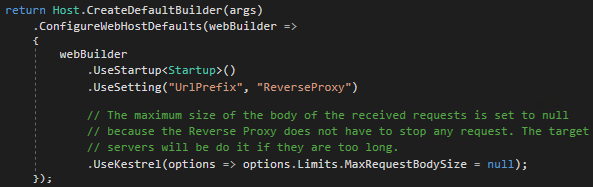
\includegraphics[width=0.9\textwidth]{imagenes/configuracionKestrel}
\caption{Esquema de dos niveles de \emph{proxy} inverso.}
	\label{configuracionKestrel}
\end{figure}

			%%%%%%%%%%%%%%%%%%%%%%%%%%%%%% RECORRIDO PETICIONES %%%%%%%%%%%%%%%%%%%%%%%%%%%%%%

			\subsubsection{Recorrido peticiones}

Una vez comentadas todas la funcionalidades del producto desarrollado se quiere mostrar un esquema (figura \ref{esquemaInteraccionProxyInverso}) del recorrido completo de una petición que proviene de la interfaz de usuario y que pasa por varios microservicios. De esta forma, se pretende ilustrar la función del \emph{proxy} inverso y cómo el resto de componentes de la aplicación interactúa con él. Entrando en detalle, la interfaz de usuario realiza una petición al microservicio 1 y para ello primero pasa por el \emph{proxy} inverso general y después por el concreto del servidor que contiene el microservicio en cuestión. Para poder responder, el microservicio 1 necesita hacer una petición al A y este, a su vez, al Z. Una vez terminadas estas peticiones anidadas, la respuesta le llega al microservicio 1 y este devuelve a la interfaz la respuesta a la petición primera. Para finalizar, es interesante resaltar el uso de los \emph{proxy} inversos tanto para las peticiones de la interfaz de usuario como para las que se realizan entre microservicios, es decir, nadie se comunica con nadie sin pasar por alguno de ellos.

\begin{figure}[ht]
\centering
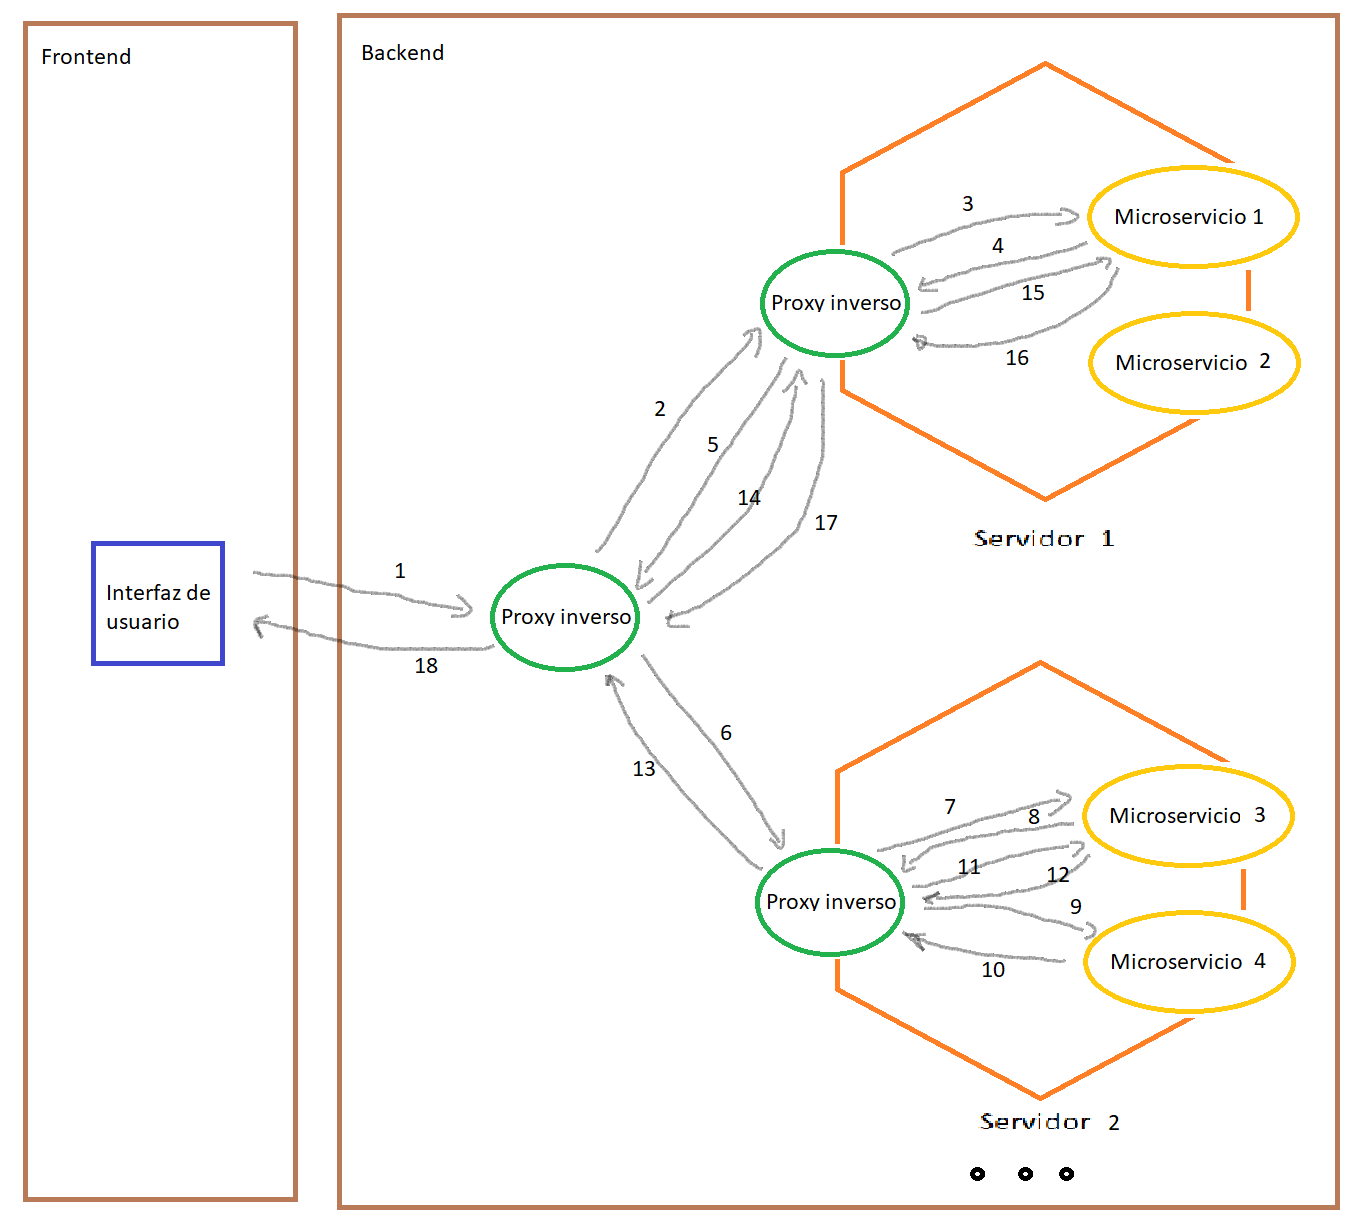
\includegraphics[width=0.9\textwidth]{imagenes/esquemaInteraccionProxyInverso}
\caption{Esquema de interacción entre el \emph{proxy} inverso y el resto de componentes de la aplicación al procesar una petición de la interfaz de usuario.}
	\label{esquemaInteraccionProxyInverso}
\end{figure}

	%%%%%%%%%%%%%%%%%%%%%%%%%%%%%% PRUEBAS %%%%%%%%%%%%%%%%%%%%%%%%%%%%%%

	\section{Pruebas} \label{pruebas}

Es interesante destacar que los despliegues comentados en el apartado de programación anterior (\ref{programacion}) se pueden considerar pruebas alfa. En ellos se introduce el \emph{proxy} inverso en el entorno en el que finalmente va a trabajar para ver cómo responde a medida que se le añaden funcionalidades. Se trata, sin duda, de pruebas que pretenden observar el comportamiento del producto \emph{software} y ver si ocurre algún fallo o problema. Como han sido detalladas en dicho apartado no cabe mencionar gran cosa más acerca de ellas, simplemente enfatizar que sirvieron para descubrir pequeños errores tales como el de los \emph{timeouts} grandes o el de las peticiones pesadas. Ambos hacían que las peticiones enrutadas no terminaran correctamente y gracias a estas pruebas se pudieron solucionar antes de dar por finalizado el proyecto.

Estas pruebas realizadas durante el desarrollo tienen un porqué. Este es el hecho de querer seguir la práctica ágil de entregas continuas, comentada en la sección \ref{metodologia}, con el fin de obtener \emph{feedback} continuo acerca del grado de corrección del \emph{proxy} inverso sobre lo que se espera de él. De esta forma, se ha considerado imprescindible no dejar las pruebas para el final, puesto que se trata de un componente clave en la arquitectura de la aplicación de la que forma parte.

Desde una perspectiva diferente a las pruebas de puesta en funcionamiento real recién descritas, se han llevado a cabo otro tipo de ellas para comprobar el correcto funcionamiento del \emph{proxy} inverso: pruebas de aceptación y pruebas de regresión. De la misma manera, han sido ejecutadas durante el desarrollo en lugar de al final de este y serán comentadas con más detalle a continuación. También es conveniente resaltar se ha utilizado consultas Postman para realizar algunas de las pruebas, por lo que estas han sido actualizadas y se ha ido creando otras a medida que se han añadido nuevas características.

		%%%%%%%%%%%%%%%%%%%%%%%%%%%%%% PRUEBAS DE ACEPTACIÓN %%%%%%%%%%%%%%%%%%%%%%%%%%%%%%

		\subsection{Pruebas de aceptación} \label{pruebasDeAceptacion}

Recordando lo comentado en el apartado \ref{metodologia}, se han definido pruebas de aceptación (PA) para especificar muchas de las unidades de trabajo que representan el trabajo a realizar. Estas determinan el buen o mal funcionamiento de la característica descrita por la unidad de trabajo en cuestión por lo que se utilizan para comprobar si esta se ha implementado correctamente.

Una unidad de trabajo no se considera terminada hasta que no pasa satisfactoriamente las pruebas de aceptación que tiene asignadas. Así pues, las pruebas de aceptación han sido ejecutadas cuando se ha creído que la unidad de trabajo a la cual hacen referencia ha estado correctamente implementada y como paso previo a incluirla en el grupo de las terminadas. En caso de no obtener un resultado positivo, estas se pasaban de nuevo una vez corregido el problema, pudiéndose repetir este proceso más de una vez.

A continuación, se va a mostrar una parte de las pruebas de aceptación elaboradas partiendo del nombre de la unidad de trabajo que prueban. Cabe destacar que, además, se han automatizado algunas de las más importantes para facilitar así su ejecución. Se enseñará también el código de alguna de ellas.

			%%%%%%%%%%%%%%%%%%%%%%%%%%%%%% DEFINICIÓN DE ALGUNAS PAs %%%%%%%%%%%%%%%%%%%%%%%%%%%%%%

			\subsubsection{Definición de algunas PAs}

Las figuras \ref{PAsAñadirRutasDinamicamente}, \ref{PAsNormalizarRutaBasePeticiones}, \ref{PAsEnrutamiento}, \ref{PAsPersonalizacionTimeouts} y \ref{PAsMultiinstanciaDeMicroservicios} son capturas de pantalla de las pruebas de aceptación de cuatro unidades de trabajo. Para cada PA se indica un nombre que la identifica, un primer punto con la acción o acciones que hay que llevar a cabo para ejecutarla y otro punto con el resultado esperado.

\begin{figure}[ht]
\centering
\includegraphics[width=0.7\textwidth]{imagenes/PAsAñadirRutasDinamicamente}
\caption{Pruebas de aceptación de la unidad de trabajo ''Añadir rutas dinámicamente''.}
	\label{PAsAñadirRutasDinamicamente}
\end{figure}

\begin{figure}[ht]
\centering
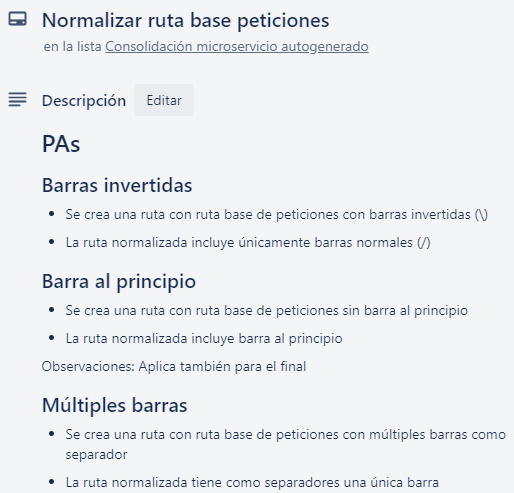
\includegraphics[width=0.7\textwidth]{imagenes/PAsNormalizarRutaBasePeticiones}
\caption{Pruebas de aceptación de la unidad de trabajo ''Normalizar rutas base peticiones''.}
	\label{PAsNormalizarRutaBasePeticiones}
\end{figure}

\begin{figure}[ht]
\centering
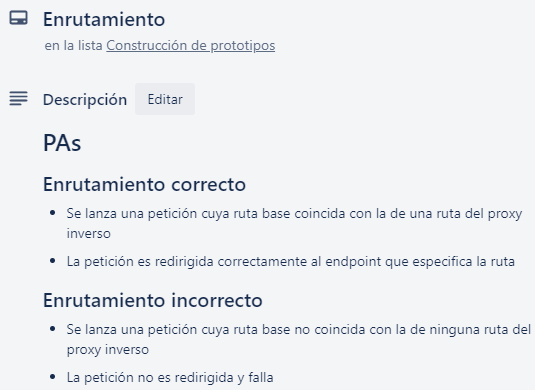
\includegraphics[width=0.7\textwidth]{imagenes/PAsEnrutamiento}
\caption{Pruebas de aceptación de la unidad de trabajo ''Enrutamiento''.}
	\label{PAsEnrutamiento}
\end{figure}

\begin{figure}[ht]
\centering
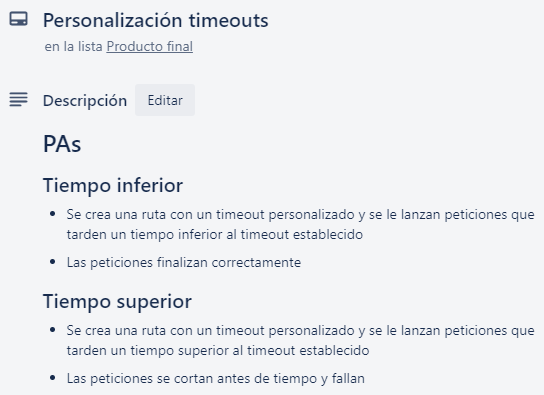
\includegraphics[width=0.7\textwidth]{imagenes/PAsPersonalizacionTimeouts}
\caption{Pruebas de aceptación de la unidad de trabajo ''Personalización timeouts''.}
	\label{PAsPersonalizacionTimeouts}
\end{figure}

\begin{figure}[ht]
\centering
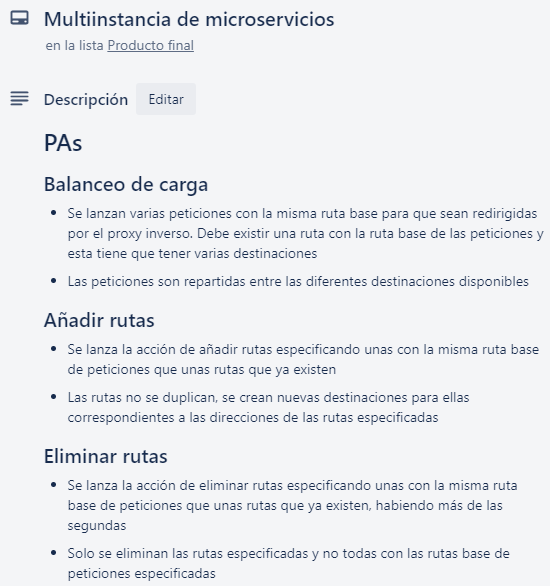
\includegraphics[width=0.7\textwidth]{imagenes/PAsMultiinstanciaDeMicroservicios}
\caption{Pruebas de aceptación de la unidad de trabajo ''Multiinstancia de microservicios''.}
	\label{PAsMultiinstanciaDeMicroservicios}
\end{figure}

			%%%%%%%%%%%%%%%%%%%%%%%%%%%%%% PRUEBAS AUTOMATIZADAS %%%%%%%%%%%%%%%%%%%%%%%%%%%%%%

			\subsubsection{Pruebas automatizadas}

Las figuras \ref{testAñadirRutas}, \ref{testGetYarpNormalizedRequestsBasePath} y \ref{testsEnrutamiento} muestran el código de algunas de las pruebas de aceptación automatizadas. Es interesante mencionar que corresponden a PAs cuyas descripciones se han enseñado en la sección anterior, figuras \ref{PAsAñadirRutasDinamicamente}, \ref{PAsNormalizarRutaBasePeticiones} y \ref{PAsEnrutamiento} en concreto. Así pues, se puede observar cómo se han automatizado y reflejado en código para entenderlas mejor.

\begin{figure}[ht]
\centering
\includegraphics[width=1\textwidth]{imagenes/testAñadirRutas}
\caption{Prueba de aceptación automatizada de la unidad de trabajo ''Añadir rutas dinámicamente''.}
	\label{testAñadirRutas}
\end{figure}

\begin{figure}[ht]
\centering
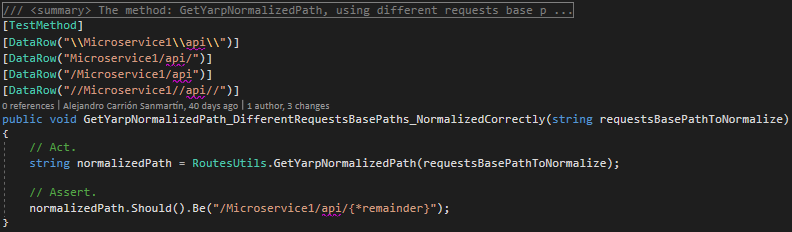
\includegraphics[width=1\textwidth]{imagenes/testGetYarpNormalizedRequestsBasePath}
\caption{Pruebas de aceptación automatizadas de la unidad de trabajo ''Normalizar rutas base peticiones''.}
	\label{testGetYarpNormalizedRequestsBasePath}
\end{figure}

\begin{figure}[ht]
\centering
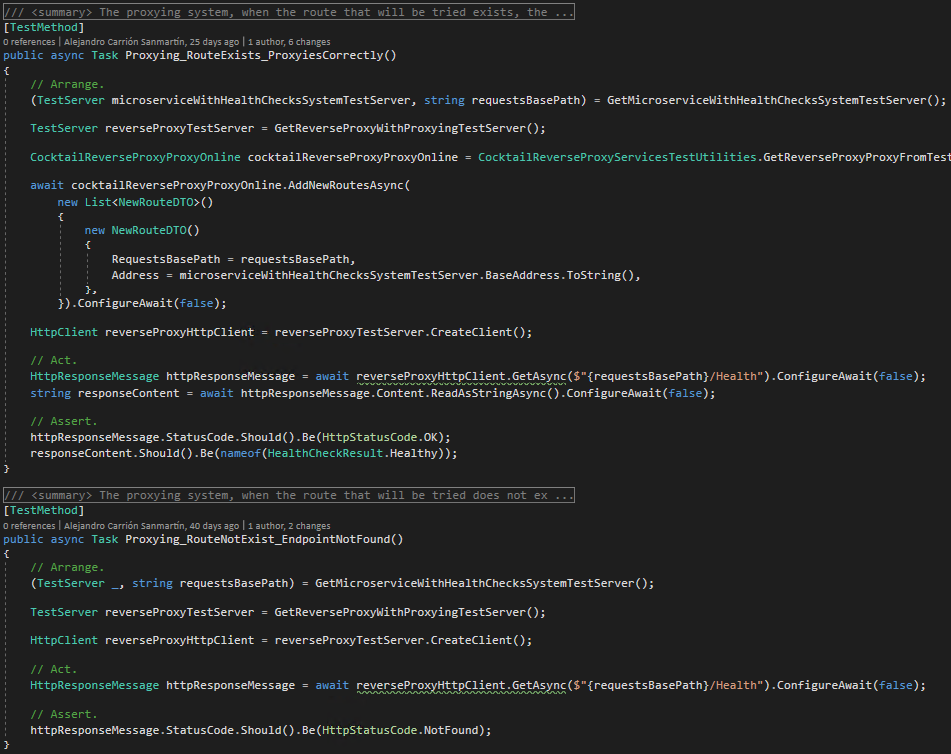
\includegraphics[width=1\textwidth]{imagenes/testsEnrutamiento}
\caption{Pruebas de aceptación automatizadas de la unidad de trabajo ''Enrutamiento''.}
	\label{testsEnrutamiento}
\end{figure}

		%%%%%%%%%%%%%%%%%%%%%%%%%%%%%% PRUEBAS DE REGRESIÓN %%%%%%%%%%%%%%%%%%%%%%%%%%%%%%

		\subsection{Pruebas de regresión} \label{pruebasDeRegresion}

Las pruebas de regresión son pruebas que se realizan sobre un producto \emph{software} anteriormente probado al que se le han hecho modificaciones. Con ellas se pretende asegurarse de que no se han introducido defectos que puedan producir errores sobre las funcionalidades implementadas previamente. 

En el caso del \emph{proxy} inverso, han consistido en ejecutar todas las pruebas de aceptación de las unidades de trabajo ya terminadas. Se han ejecutado antes de cada despliegue y con ellas se ha verificado el correcto funcionamiento de todas las características del producto de cara a que los despliegues no hicieran fallar el \emph{proxy} inverso ni cualquier otro componente de la aplicación. De esta forma, con estas pruebas se ha pretendido evitar todo tipo de problemas que pudieran entorpecer a los demás miembros del equipo de desarrollo de la aplicación ya que, si el \emph{proxy} inverso quedara caído durante un tiempo, el resto de microservicios y la interfaz de usuario no podrían contactar con nadie y caerían también. Es por esto que se han considerado un seguro de vida para garantizar, en cierta medida, que los despliegues serían un éxito.

%%%%%%%%%%%%%%%%%%%%%%%%%%%%%% CONCLUSIONES Y TRABAJO FUTURO %%%%%%%%%%%%%%%%%%%%%%%%%%%%%%

\chapter{Conclusiones y trabajo futuro}

El resultado de este proyecto es un \emph{proxy} inverso totalmente funcional, capaz de cubrir las
necesidades planteadas y actuar correctamente en los casos de uso para los que fue concebido. De esta manera, todos los requisitos, tanto funcionales como no funcionales, han sido cubiertos satisfactoriamente. A pesar de ello, es necesario decir que algunas funcionalidades se podrían haber mejorado si no fuera por el hecho de que las partes de la aplicación con las que se integra el \emph{proxy} inverso no están acabadas al tratarse de una aplicación en desarrollo. Por ejemplo, el microservicio encargado de orquestar los despliegues no está cien por cien operativo todavía.

Desde otra perspectiva, el producto resultante también cumple los objetivos inicialmente definidos. El \emph{proxy} inverso logra ocultar los microservicios, haciendo que la interfaz de usuario no conozca donde se encuentran y no acceda directamente a ellos. Permite, además, la ejecución de más de una instancia de un mismo microservicio, otorgando así cierta tolerancia a fallos y aumentando la eficiencia de la aplicación.

A pesar de haber cumplido los objetivos, es interesante hacer una breve reflexión para reconocer los aspectos negativos del producto desarrollado. Así pues, el \emph{proxy} inverso constituye un nuevo punto único de fallo, además de tener la posibilidad de actuar como cuello de botella, ralentizando las peticiones de toda la aplicación. Sin embargo, estos dos aspectos se han combatido permitiendo la existencia de más de una instancia del \emph{proxy} inverso. Por otra parte, un asunto al cual no se le a dado solución es el hecho de que los \emph{middleware} construidos para la \emph{pipeline} de YARP aumentan el tiempo de respuesta de las peticiones. No obstante, no se supera el límite definido por el requisito no funcional RNF02, en el apartado \ref{requisitosNoFuncionales}.

En lo referente a los conocimientos necesarios para la ejecución de este proyecto, es interesante comentar que el lenguaje de programación utilizado, C\#, es visto en los estudios en los que se enmarca este trabajo, si bien, no con la profundidad suficiente para poder abordar un problema de estas características. Además, no es lo mismo hacer programas de escritorio con Windows Forms \cite{WinForms} como \emph{framework}, que es lo enseñado en ellos principalmente, que aplicaciones de tipo servicio web. Por otra parte, las asignaturas de metodología \emph{software} y de sistemas en red también han resultado una muy buena base. Las primeras han servido para establecer y seguir una disciplina de desarrollo acorde a las características del proyecto y a su contexto. Las segundas, para entender mejor el funcionamiento de las comunicaciones entre varios servicios y del propio \emph{proxy} inverso. Por último, YARP es una librería con un propósito muy específico, por lo que su aprendizaje ha requerido cierto esfuerzo, sobre todo para poder utilizar algunas de sus características más avanzadas.

Por lo que se refiere a experiencia personal, ha sido muy gratificante llevar a cabo este trabajo. Por un lado, ha servido como ensayo para la futura resolución de problemas mayores en el mundo laboral, aunque también se pueda interpretar este como un trabajo profesional al haberse realizado en el contexto de una empresa. Por otro, ha merecido la pena este último hecho, pues ha otorgado cierta confianza dentro de la propia organización y se cree que con un proyecto real el proceso de aprendizaje ha sido más fructífero, teniendo en cuenta las desventajas que conlleva.

En cuanto a líneas de trabajo futuras, el \emph{proxy} inverso quizás requiera alguna nueva característica o modificación que otra a medida que el resto de la aplicación avance y surjan nuevas necesidades. Para finalizar, también se puede querer extender la funcionalidad más adelante y construir encima un API \emph{Gateway} que ofrezca características específicas de ese patrón. Estas pueden ser agregaciones de peticiones o tareas transversales tales como monitorización de tiempos de las peticiones.

%%%%%%%%%%%%%%%%%%%%%%%%%%%%%% REFERENCIAS %%%%%%%%%%%%%%%%%%%%%%%%%%%%%%

\renewcommand{\bibname}{Referencias}

\begin{thebibliography}{10}

\bibitem{DevOps}
¿Qué es DevOps? (consultado en 08/2021):\\
\url{https://azure.microsoft.com/es-es/overview/what-is-devops}.

\bibitem{DevOpsPracticas}
Integración y entrega continua (consultado en 08/2021):\\
\url{https://azure.microsoft.com/es-es/overview/what-is-devops/#practices}

\bibitem{Microservicios_articulo}
\newblock \emph{Microservices}.
\newblock J. Lewis y M. Fowler, 2014 (consultado en 08/2021):\\
\url{https://martinfowler.com/articles/microservices.html}

\bibitem{Microservicios_libro}
\newblock \emph{Building Microservices}.
\newblock S. Newman, O'REILLY, 2015.
\newblock ISBN: 9781491950357

\bibitem{DotNetCore}
Documentación oficial de ASP.NET Core (consultado en 08/2021):\\
\url{https://docs.microsoft.com/es-es/aspnet/core/?view=aspnetcore-5.0}

\bibitem{ApiGateway}
Uso de puertas de enlace de API (API \emph{Gateway}) en microservicios (consultado en 08/2021):\\
\url{https://docs.microsoft.com/es-es/azure/architecture/microservices/design/gateway}

\bibitem{NGINX}
Web oficial de NGINX (consultado en 08/2021):\\
\url{https://www.nginx.com}

\bibitem{NGINX_documentacion}
Documentación oficial de NGINX para funcionar como \emph{proxy} inverso (consultado en 08/2021):\\
\url{https://docs.nginx.com/nginx/admin-guide/web-server/reverse-proxy}

\bibitem{Ocelot_documentacion}
Documentación oficial de Ocelot (consultado en 08/2021):\\
\url{https://ocelot.readthedocs.io}

\bibitem{OSI}
¿Qué es el modelo OSI? (consultado en 08/2021):\\
\url{https://www.ionos.es/digitalguide/servidores/know-how/el-modelo-osi-un-referente-para-normas-y-protocolos}

\bibitem{MiddlewaresPipeline}
El método \emph{Configure} y la \emph{pipeline} de \emph{middlewares} (consultado en 08/2021):\\
\url{https://docs.microsoft.com/es-es/aspnet/core/fundamentals/startup?view=aspnetcore-5.0#the-configure-method}

\bibitem{DotNet}
Documentación oficial de .NET (consultado en 08/2021):\\
\url{https://docs.microsoft.com/es-es/dotnet}

\bibitem{Csharp}
Documentación oficial de C\# (consultado en 08/2021):\\
\url{https://docs.microsoft.com/es-es/dotnet/csharp}

\bibitem{NuGet}
Una introducción a NuGet (consultado en 08/2021):\\
\url{https://docs.microsoft.com/es-es/nuget/what-is-nuget}

\bibitem{ISO25010}
\emph{System and software Quality Requirements and Evaluation}, ISO/IEC 25010 (consultado en 08/2021):\\
\url{https://iso25000.com/index.php/normas-iso-25000/iso-25010}

\bibitem{Kestrel}
Implementación del servidor web Kestrel en ASP.NET Core (consultado en 08/2021):\\
\url{https://docs.microsoft.com/es-es/aspnet/core/fundamentals/servers/kestrel}

\bibitem{WinForms}
Guía de escritorio, .NET para Windows Forms (consultado en 08/2021):\\
\url{https://docs.microsoft.com/es-es/dotnet/desktop/winforms/overview}

\end{thebibliography}

%%%%%%%%%%%%%%%%%%%%%%%%%%%%%% APÉNDICE %%%%%%%%%%%%%%%%%%%%%%%%%%%%%%

\APPENDIX

\chapter{Proceso de generación automática de código}

A lo largo de toda la memoria se ha mencionado el hecho de que la aplicación de la que forma parte el \emph{proxy} inverso, y finalmente él mismo también, se ha construido utilizando técnicas de generación automática de código a partir de modelos. Sin embargo, no se ha entrado en mucho más detalle ya que no se ha considerado imprescindible y no se ha querido desviar la atención del producto desarrollado. De esta forma, este apéndice está destinado a complementar la información dada hasta ahora, explicando y dando ejemplos para el caso particular, del proceso de generación automática de código que se ha seguido para elaborar el \emph{proxy} inverso.

El proceso en cuestión se divide en 3 pasos que se repiten continuamente en un proceso iterativo e incremental.

También se modelan interfaces de usuario pero el \emph{proxy} inverso no lo requiere.
En general, el modelado para el \emph{proxy} inverso es muy simple.

	\section{Modelado}

Entidades, DTOs y acciones \emph{ad hoc}.
Utilizando los modelos de Dominio y Aplicación. Existen más pero no conviene marear, por simplicidad. 
Esta parte consiste en utilizar las herramientas de modelado, llamadas DSL Tools. Primero de todo, es necesario construir las entidades que representan el dominio de la aplicación, microservicio en este caso. Para ello se crean modelos de dominio.
Una vez creados los modelos de dominio, hay que modelar las acciones ad hoc. Estas representan las funcionalidades que el microservicio va a tener.

	\section{Generación de código}

Se ejecuta mediante un \emph{script}.
Generar código a partir de los modelos. Se genera buena parte de la infraestructura de un microservicio.
Como se ha visto en el apartado ??????, la arquitectura generada es una arquitectura por capas que trata de seguir siempre buenos principios de programación comos los SOLID.

Referenciar documentación interna de la empresa.

	\section{Programación de particularidades}

Se implementan a través de clases parciales.
No todo el código se puede generar automáticamente. Es necesaria la intervención humana para programar cosas concretas como campos calculados, validaciones o acciones ad hoc.

\end{document}
